\documentclass[a4paper,11pt,fullpage,oneside,openany]{amsbook}
\usepackage[utf8]{inputenc}
\usepackage{graphicx}
\usepackage{mathrsfs}
\usepackage{amsbsy}
\usepackage{fontenc}
\usepackage{amsfonts}
\usepackage{amsmath} 	
\usepackage{mdframed}
\usepackage{amsthm}  	
\usepackage{amssymb}
\usepackage{amscd}
\usepackage{faktor}
\usepackage{mathtools}
\usepackage{epigraph}
\usepackage{tikz}
\usetikzlibrary{matrix,arrows,decorations.pathmorphing}
\usepackage{tikz-cd}
\usepackage[titletoc]{appendix}
\usepackage{centernot}
\usepackage{bbding}
\usepackage{indentfirst}
\usepackage{hyperref}
\usepackage{xspace}
\hypersetup{colorlinks=false, pdfborder={0 0 0}}                                 
\usepackage{enumitem}
\setdescription{font=\normalfont}
\usepackage[type={CC}, modifier={by-nc-sa}, version={4.0}]{doclicense}
%\usepackage[style=alphabetic, backend=bibtex]{biblatex}
\usepackage[normalem]{ulem}
\usepackage{contour}
\usepackage{fullpage}
\makeatletter        
\newcommand*{\doublerightarrow}[2]{\mathrel{
		\settowidth{\@tempdima}{$\scriptstyle#1$}
		\settowidth{\@tempdimb}{$\scriptstyle#2$}
		\ifdim\@tempdimb>\@tempdima \@tempdima=\@tempdimb\fi
		\mathop{\vcenter{
				\offinterlineskip\ialign{\hbox to\dimexpr\@tempdima+1em{##}\cr
					\rightarrowfill\cr\noalign{\kern.5ex}
					\rightarrowfill\cr}}}\limits^{\!#1}_{\!#2}}}
\newcommand*{\triplerightarrow}[1]{\mathrel{
		\settowidth{\@tempdima}{$\scriptstyle#1$}
		\mathop{\vcenter{
				\offinterlineskip\ialign{\hbox to\dimexpr\@tempdima+1em{##}\cr
					\rightarrowfill\cr\noalign{\kern.5ex}
					\rightarrowfill\cr\noalign{\kern.5ex}
					\rightarrowfill\cr}}}\limits^{\!#1}}}
\makeatother

\def\cleardoublepage{\clearpage\if@twoside \ifodd\c@page\else  		
	\hbox{}                                                        					
	\vspace*{\fill}                                                					
	\begin{center}                                                 					
		\*                                                             					
	\end{center}                                                   					
	\vspace{\fill}                                                 					 
	\thispagestyle{empty}                                          				
	\newpage                                                       					
	\if@twocolumn\hbox{}\newpage\fi\fi\fi}                        

\makeatletter
\newcommand{\colim@}[2]{%
	\vtop{\m@th\ialign{##\cr
			\hfil$#1\operator@font colim$\hfil\cr
			\noalign{\nointerlineskip\kern-\ex@}\cr}}%
}
\newcommand{\colim}{%
	\mathop{\mathpalette\colim@{\rightarrowfill@\scriptscriptstyle}}\nmlimits@
}

\newcommand\Yoneda{\mathrel{\overset{\makebox[0pt]{\mbox{\normalfont\tiny\sffamily Yoneda}}}{\cong}}}

\newcommand{\catname}[1]{{\normalfont\textbf{#1}}}

\DeclareMathOperator{\Aff}{\mathbf{Aff}}
\DeclareMathOperator{\Alg}{\mathbf{Alg}}
\DeclareMathOperator{\Coh}{\mathbf{Coh}}
\DeclareMathOperator{\QCoh}{\mathbf{QCoh}}
\DeclareMathOperator{\VB}{\mathbf{VB}}
\DeclareMathOperator{\Arr}{Arr}

\newcommand{\Set}{\catname{Set}}
\newcommand{\Top}{\catname{Top}}
\newcommand{\CHTop}{\catname{CHTop}}
\newcommand{\Ab}{\catname{Ab}}
\newcommand{\RMod}{\catname{Mod}_R}
\newcommand{\sSet}{\catname{sSet}}
\newcommand{\Rel}{\catname{Rel}}
\newcommand{\Cat}{\catname{Cat}}
\newcommand{\CAT}{\catname{CAT}}	
\newcommand{\qCat}{\catname{qCat}}	
\newcommand{\yo}{\text{\usefont{U}{min}{m}{n}\symbol{'210}}}
\newcommand{\from}{\colon}
\newcommand{\card}[1]{\left\lvert #1 \right\rvert}
\makeatother                                                   

\DeclareFontFamily{U}{min}{}
\DeclareFontShape{U}{min}{m}{n}{<-> udmj30}{}

\makeatletter
\renewcommand\part{%
	\if@openright
	\cleardoublepage
	\else
	\clearpage
	\fi
	\thispagestyle{empty}%  				 
	\if@twocolumn
	\onecolumn
	\@tempswatrue
	\else
	\@tempswafalse
	\fi
	\null\vfil
	\secdef\@part\@spart}
\makeatother
\usepackage{bbm}
\usepackage{fancyhdr}                                   	

\renewcommand{\sectionmark}[1]{\markright{#1}}         	         
\pagestyle{fancy}                                       				
\fancyhf{}                                              				
\fancyhead[LE,RO]{\thepage}                           		           
\fancyhead[LO]{\scshape\nouppercase{\rightmark}}       	          
\fancyhead[RE]{\scshape\nouppercase{\leftmark}}      	           
\renewcommand{\headrulewidth}{0pt}                   \usepackage{amsmath,calligra,mathrsfs}
\DeclareMathOperator{\innerhom}{\mathscr{H}\text{\kern -3pt {\calligra\Large om}}\,}
\DeclareMathOperator{\Hom}{\text{Hom}}
\DeclareMathOperator{\End}{\text{End}}
\DeclareMathOperator{\op}{\text{op}}
\DeclareMathOperator{\co}{\text{co}}
\DeclareMathOperator{\coop}{\text{coop}}
\DeclareMathOperator{\Fib}{\text{Fib}}
\DeclareMathOperator{\Cof}{\text{Cof}}
\DeclareMathOperator{\V}{\mathcal{V}}
\DeclareMathOperator{\A}{\mathbf{A}}
\DeclareMathOperator{\B}{\mathbf{B}}
\DeclareMathOperator{\C}{\mathbf{C}}
\DeclareMathOperator{\D}{\mathbf{D}}
\DeclareMathOperator{\I}{\mathbf{I}}
\DeclareMathOperator{\J}{\mathbf{J}}
\DeclareMathOperator{\N}{\mathbb{N}}
\DeclareMathOperator{\Z}{\mathbb{Z}}
\DeclareMathOperator{\id}{id}
\DeclareMathOperator{\dom}{dom}
\DeclareMathOperator{\cod}{cod}
\DeclareMathOperator{\Ob}{Ob}
\DeclareMathOperator{\Ar}{Ar}
\DeclareMathOperator{\Lan}{Lan}
\DeclareMathOperator{\Cone}{Cone}
\DeclareMathOperator{\Cocone}{Cocone}
\DeclareMathOperator{\Nat}{Nat}

\tikzset{shorten <>/.style={shorten >=#1,shorten <=#1}}
\newcommand{\pullbackcorner}[1][ul]{\save*!/#1+1.5pc/#1(1,-1)@^{|-}\restore}
\newcommand{\pushoutcorner}[1][ul]{\save*!/#1-1.5pc/#1:(-1,1)@^{|-}\restore}
\usepackage{tikz}
\usetikzlibrary{shapes}
\usepackage{xcolor}
\usepackage{url}
\usepackage{attachfile} 							
\makeatletter                        						
\g@addto@macro{\UrlBreaks}{\UrlOrds} 				
\makeatother                        						 
\usepackage{xcolor}
\usepackage{url}
\usepackage{attachfile} 							


\makeatletter                        						

\g@addto@macro{\UrlBreaks}{\UrlOrds} 				

\makeatother                        						 

\newsavebox\MBox

\newcommand\Cline[2][red]{{\sbox\MBox{$#2$}%
		
		\rlap{\usebox\MBox}\color{#1}\rule[-1.2\dp\MBox]{\wd\MBox}{1pt}}}

\theoremstyle{definition}

\newtheorem{thm}{Theorem}[section] % reset theorem numbering for each chapter

\newcommand{\chaptercontent}{
	\section{Basics}
	\begin{defn}Here is a new definition.\end{defn}
	\begin{thm}Here is a new theorem.\end{thm}
	\begin{exmp}Here is a good example.\end{exmp}
	\subsection{Some tips}
	\begin{defn}Here is a new definition.\end{defn}
	\section{Advanced stuff}
	\begin{defn}Here is a new definition.\end{defn}
	\subsection{Warnings}
	\begin{defn}Here is a new definition.\end{defn}
}
\theoremstyle{definition}
\newtheorem{defn}[thm]{Definition} % definition numbers are dependent on theor$
\newtheorem{exmp}[thm]{Example} % same for example numbers
\newtheorem{prop}[thm]{Proposition}
\newtheorem{lemma}[thm]{Lemma}
\newtheorem{cor}[thm]{Corollary}
\theoremstyle{remark}
\newtheorem{rmk}[thm]{Remark}
\newtheorem{es}[thm]{Example}

\newmdtheoremenv{theo}[thm]{Theorem}

\newmdtheoremenv{teo}{Theorem}

\setlength{\headheight}{15pt} 					  
\usepackage[all]{xy}
\usepackage{extarrows}


\begin{document}
	\begin{titlepage}
		\begin{center}
			\Huge \bf{Monads~and~their~applications}\\
			\vspace{1cm}
			\Large Dr.\ Daniel Schäppi's course lecture notes\\
		\end{center}
		
		\vspace{1cm}

			\begin{center}
			\Large	by\\
				\vspace{.2cm}
			\Large	Nicola Di Vittorio\\
			\Large	Matteo Durante 
		
\vspace{1.5cm}
\begin{figure}[!b]
	\centering
	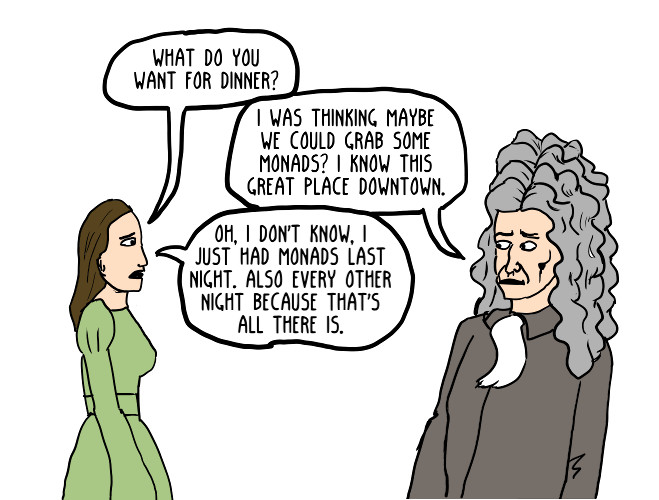
\includegraphics[scale=.7]{monadsForDinner.jpg}\\
	%\vspace{.3cm}
	%\includegraphics[scale=.3]{intbn}
\end{figure}	
\end{center}
		
	\end{titlepage}


\frontmatter
	\thispagestyle{empty}\doclicenseThis
	Cover image \copyright \href{http://existentialcomics.com/comic/other/10}{\ Existential comics}
	\tableofcontents
	
	\mainmatter
	
	\chapter*{Categorical preliminaries}
	\begin{defn}[Categories]
		A \emph{category} $\C$ consists of:
		\begin{enumerate}
			\item a collection of objects $\Ob(\C)$;
			\item a collection of arrows $\Ar(\C)$;
			\item two maps $\dom,\cod\colon\Ar(\C)\rightarrow\Ob(\C)$;
			\item a map $\id_{-}\colon\Ob(\C)\rightarrow\Ar(\C)$ with $\dom(\id_{c})=c=\cod(\id_{c})$;
			\item for every $f,g\in\Ar(\C)$ such that $\cod(f)=\dom(g)$ a unique composite morphism $gf$ such that $\cod(gf)=\cod(g)$, $\dom(gf)=\dom(f)$.
		\end{enumerate}
	This data has to satisfy the following axioms
		\begin{enumerate}
			\item given $f\in\Ar(\C)$, $c=\dom(f)$ and $c'=\cod(f)$, $\id_{c'}f=f=\id_{c}$, that is the composition is unital;
			\item given a composable triple $f,g,h\in\Ar(\C)$, $h(gf)=(hg)f$, that is the composition is associative.
		\end{enumerate}
		An arrow $f$ such that $c=\dom(f)$ and $c'=\cod(f)$ is denoted $f\colon c\rightarrow c'$.
	\end{defn}
	
	\begin{defn}[Functors]
		
	\end{defn}
	
	\begin{defn}[Full functors, faithful functor]
		
	\end{defn}
	
	\begin{defn}[Natural transformations]
		
	\end{defn}
	
	\begin{defn}[Equivalent functors]
	\end{defn}
	
	\begin{defn}[Representable Functors]
		
	\end{defn}
	
	\begin{defn}[Whiskering]
		
	\end{defn}
	
	\begin{defn}[Horizontal and vertical composition of nat.transf.]
		
	\end{defn}
	
	\begin{defn}[adjunctions]
		
	\end{defn}
	
	\begin{lemma}[Yoneda]
		
	\end{lemma}
	\begin{proof}
		
	\end{proof}

\noindent We will denote by $\yo$  (the hiragana kata for ``Yo'') the Yoneda embedding $\C\hookrightarrow\Set^{\C^{\op}}$.
	
	\chapter{Monads and algebras}
	
	\section{Introduction}
		
	Throughout mathematics we encounter structures defined by some action morphisms. Here we give some examples.
	
	\begin{exmp}
		Given a group $G$, we may consider a $G$-set $X$ described by an action map $G\times X\rightarrow X$.
	\end{exmp}
	\begin{exmp}
		Given an abelian group $M$ and a ring $R$, we can get an $R$-module $M$ by fixing a group homomorphism $R\otimes_{\Z} M\rightarrow M$.
	\end{exmp}
	\begin{exmp}
		Given a monoid $M$ in $\Set$, we get a map $\Pi_{k=1}^n M\rightarrow M$, $(m_1,\ldots,m_n)\mapsto ((\ldots ((m_1m_2)m_3)\ldots )m_{n-1}) m_n$. This induces an action map from $W(M)=\amalg_{n\in\N}\Pi_{k=1}^n M$, the set of words on $M$, to $M$.
	\end{exmp}
	\begin{exmp}\label{ultrafilters}
		Given a set $X$, let $\mathcal{U}X$ be the set of ultrafilters on it. Any compact T2 topology on $X$ allows us to see each ultrafilter as a system of neighborhoods of a unique point in $X$, hence it gives us a unique map $\mathcal{U}X\rightarrow X$ sending each ultrafilter to the respective point.
	\end{exmp}
	\begin{exmp}
		Given a directed graph $D=(V,E,\hspace{-1.5mm}\begin{tikzcd}
		E\hspace{-1.5mm}\arrow[r, "t" description,  shift right=.5ex, shorten <= .3em, shorten >= .3em]  \arrow[r, "s" description, shift left=1ex, shorten <= .3em, shorten >= .3em] & \hspace{-1.5mm}V
		\end{tikzcd}\hspace{-1.5mm})$, we can create its free category $FD$, where the objects are the vertices and $FD(v,w)=\{\text{finite paths } v\rightarrow\ldots\rightarrow w\}$. We set $\id_v$ to be the path of length 0, while composition is just the concatenation of paths.
		
		In particular, if $D$ is the directed graph with $V=\{0,\ldots,n\}$ and an edge $j\rightarrow k$ if and only if $k=j+1$, we have $FD\cong [n]$.
		
		If $D=\{*\}$ and $E=\{*\rightarrow *\}$, then $FD(*,*)\cong\N$.
		
		Given a small category $\C$, we may consider the underlying graph $U\C=D$ with $V=\Ob(\C)$, $E=\Ar(\C)$, $s=\dom$ and $t=\cod$. We get then an action map $UFU\C\rightarrow U\C$ sending a finite path to its composite. This map is a morphism of directed graphs.
	\end{exmp}

	Notice that we always have a category $\C$ and some functor $T\colon\C\rightarrow\C$ with an action map $T\C\rightarrow\C$. How can we see all of these examples as specific instances of a general phenomenon?
	
	\begin{defn}
		A \emph{monad} on a category $\C$ is a triple $(T,\mu,\eta)$ where $T\colon\C\rightarrow\C$ is a functor, while $\mu\colon T^2\Rightarrow T$ and $\eta\colon\id_{\C}\Rightarrow T$ are natural transformations such that the following diagrams commute.
		
		\[
			\begin{tikzcd}
				T^3\ar["\mu T"', Rightarrow]{d}\ar["T\mu", Rightarrow]{r}
				& T^2\ar["\mu", Rightarrow]{d} \\
				T^2\ar["\mu"', Rightarrow]{r}
				& T
			\end{tikzcd}
			\quad\quad
			\begin{tikzcd}
				T\ar["\eta T", Rightarrow]{r}\ar["\id_{T}", Rightarrow, swap]{dr}
				& T^2\ar["\mu", Rightarrow]{d}\ar["T\eta", Leftarrow]{r}
				& T\ar["\id_{T}", Rightarrow]{dl} \\
				& T
			\end{tikzcd}
		\]
		
		$\mu$ is called the \emph{multiplicative map}, while $\eta$ is the \emph{unit} of $T$.
		
		The commutativity of the first diagram is equivalent to stating that the following two diagrams are equal.
		\begin{center}
		\begin{minipage}{0.3\linewidth}
			\begin{tikzcd}[row sep=1cm, column sep=1cm]
				&\C\ar[d, Rightarrow, shorten <= 1em, shorten >= 1em, "\mu"]\ar[r, "T"]\ar[drr, bend right=26, "T"description]
				&\C\ar[dr, "T"]\ar[d, Rightarrow, yshift=1ex, shorten <= 1em, shorten >= 1em, "\mu"]\\
				\C
				\ar[rrr, "T"'] 
				\ar[ur, , "T"]
				&\phantom{.} &\phantom{.}&\C
			\end{tikzcd}
		\end{minipage}
		\hspace{1cm}
				=
		\hspace{.2cm}
		\begin{minipage}{0.3\linewidth}
			\begin{tikzcd}[row sep=1cm, column sep=1cm]
				&\C\ar[d, Rightarrow, yshift=1ex, shorten <= 1em, shorten >= 1em, "\mu"]\ar[r, "T"]
				&\C\ar[d, Rightarrow, shorten <= 1em, shorten >= 1em, "\mu"]\ar[dr, "T"]\\
				\C\ar[urr, bend right=26, "T"'description]
				\ar[rrr, "T"'] 
				\ar[ur, , "T"]
				&\phantom{.} &\phantom{.}&\C
			\end{tikzcd}
		\end{minipage}
		\end{center}
	\end{defn}

On the other hand, the second diagram can be rephrased as follows:
\begin{center}
	
	\begin{minipage}{0.3\linewidth}
		\begin{tikzcd}[row sep=1cm, column sep=1cm]
		& \C \arrow[d, Rightarrow, shift left=.5ex, shorten <= 1em, shorten >= 1em, "\mu"]\arrow[d, Rightarrow, shift right=5.8ex, shorten <= 1em, shorten >= 1em, "\eta"]\arrow[rd, "T"] &   \\
		\C \arrow[rr, "T"', ""{name=A}] \arrow[ru, bend right, "T"'description, ""{name=T}] \arrow[ru, bend left, equal, ""{name=U}] &    \phantom{.}          & \C
		%\arrow[Rightarrow, from=U, to=D]
		\end{tikzcd}
		
	\end{minipage}
	=
	\hspace{.4cm}
	\begin{minipage}{0.3\linewidth}
		\begin{tikzcd}[row sep=1cm, column sep=1cm]
		\C \arrow[d, bend right, "T"'] \arrow[d, bend left, "T"] \\
		\C                                           
		\end{tikzcd}
	\end{minipage}
	\hspace{-4.5cm}
	=
	\hspace{1cm}
	=
	\hspace{.6cm}
	\begin{minipage}{0.3\linewidth}
		\begin{tikzcd}[row sep=1cm, column sep=1cm]
		& \C \arrow[d, Rightarrow, shift right=1.2ex, shorten <= 1em, shorten >= 1em, "\mu"]\arrow[d, Rightarrow, shift left=5.8ex, shorten <= 1em, shorten >= 1em, "\eta"] \arrow[rd, bend right, "T"'description, ""{name=T}] \arrow[rd, bend left, equal, ""{name=U}] &   \\
		\C \arrow[rr, "T"', ""{name=A}] \arrow[ru, "T", ""{name=B}] &\phantom{.}   & \C		\end{tikzcd}
	\end{minipage}
\end{center}

	A monad naturally defines other algebraic structures, which we now introduce.
	
	\begin{defn}
		Given a monad $(T,\mu,\eta)$, a \emph{$T$-algebra} or \emph{$T$-module} is a pair $(a,\alpha)$, where $a\in\Ob(\C)$ and $\alpha\colon Ta\rightarrow a$ is such that the following diagrams commute.
		\[	
			\begin{tikzcd}
				T^2 a\ar["\mu_{a}"']{d}\ar["T\alpha"]{r}
				& Ta\ar["\alpha"]{d} \\
				Ta\ar["\alpha"']{r}
				& a
			\end{tikzcd}
			\quad\quad
			\begin{tikzcd}
				a\ar[equal, swap]{dr}\ar["\eta_{a}"]{r}
				& Ta\ar["\alpha"]{d} \\
				& a
			\end{tikzcd}
		\]
	\end{defn}

	\begin{defn}
		A \emph{morphism of $T$-algebras} $(a,\alpha)\rightarrow (b,\beta)$ is a morphism $f\colon a\rightarrow b$ such that the following diagram commutes:
		\[
			\begin{tikzcd}
				Ta\arrow["\alpha"']{d}\arrow["Tf"]{r}
				& Tb\arrow["\beta"]{d} \\
				a\arrow["f"']{r}
				& b
			\end{tikzcd}
		\]
	\end{defn}

		
	$T$-algebras form a category $T\mbox{-}\Alg$, which has a natural forgetful functor $U^T\colon T\mbox{-}\Alg\rightarrow\C$.
	
	We now show how to recover the examples previously given with this language.
	
	\begin{exmp}
		\begin{align*}
			T=G\times - \colon&\ \Set \rightarrow\Set \\
			\mu_A\colon&\ G\times (G\times A) \rightarrow G\times A \\
			&\ (g,(h,a)) \mapsto (gh,a) \\
			\eta_A\colon&\ A \rightarrow G\times A \\
			&\ a \mapsto (e,a)
		\end{align*}
		is a monad and $(A,\alpha)$ is a $T$-algebra if and only if $A$ is a $G$-set. It follows that $T\mbox{-}\Alg\cong G\mbox{-}\Set$.
	\end{exmp}

	\begin{exmp}
		Given a ring $R$, $T=R\otimes_{\Z}-\colon \Ab\rightarrow \Ab$ is a monad when considered with the following natural transformations:
		\begin{align*}
			\mu_{-}\colon &\ R\otimes_{\Z}(R\otimes_{\Z}-)\cong (R\otimes_{\Z})\otimes_{\Z}-\Rightarrow R\otimes_{\Z}- \\
			\eta_-\colon &\ -\cong\Z\otimes_{\Z}-\Rightarrow R\otimes_{\Z}-
		\end{align*}
	We have that $(R\otimes_{\Z}-)\mbox{-}\Alg\cong \RMod$.
	\end{exmp}

	\begin{exmp}
		Consider $W\colon\Set\rightarrow\Set$ given by $WX=\amalg_{n\in\N}\Pi_{k=1}^n X$. Multiplication $\mu_X\colon WWX\rightarrow WX$ is given by concatenation of words, while the unit $\eta_X\colon X\rightarrow WX$ is just $x\mapsto (x)$. With this, $W\mbox{-}\Alg\cong \text{Mon}(\Set)$.
	\end{exmp}

	\begin{exmp}
		The functor $\mathcal{U}$ defined in Example \ref{ultrafilters}, equipped with suitable natural transformations, is a monad on $\Set$ and $\mathcal{U}\mbox{-}\Alg\cong \CHTop$, the category of compact T2 spaces.
	\end{exmp}

	\begin{exmp}
		The free-forgetful adjunction $F\dashv U$ between categories and directed graphs induces a monad on the latter, with $UF\mbox{-}\Alg\cong\Cat$.
	\end{exmp}

	\section{Monadic functors}
	
	Now that we have introduced these structures, our aim is to characterize \emph{monadic functors}, that is functors $U\colon\A\rightarrow\C$ which are equivalent to $U^T\colon T\mbox{-}\Alg\rightarrow\C$ for some monad $(T,\mu,\eta)$ on $\C$.

	First of all, notice that $U^T$ is faithful by construction, hence $U$ must be faithful, but more is true.
	
	\begin{lemma}
		The functor $U^T$ is conservative, that is if $U^Tf$ is an isomorphism then $f$ is an isomorphism of $T$-algebras.
	\end{lemma}
	\begin{proof}
		Suppose that $g$ is the inverse of $f\colon a\rightarrow b$ and $f$ is a morphism $(a,\alpha)\rightarrow (b,\beta)$. We only need to prove that the square on the left commutes, that is $g\beta=\alpha Tg$:
		\[
			\begin{tikzcd}
				Tb\arrow["\beta"']{d}\arrow["Tg"]{r}
				& Ta\arrow["\alpha"']{d}\arrow["Tf"]{r}
				& Tb\arrow["\beta"]{d} \\
				b\arrow["g"']{r}
				& a\arrow["f"']{r}
				& b
			\end{tikzcd}
		\]
		
	We see that $fg\beta=\beta$ and $f\alpha Tg=\beta Tf Tg=\beta T(fg)=\beta T\id_b=\beta$, hence the thesis.
	\end{proof}
    \begin{rmk}
     Notice that the forgetful functor $U\colon\Top\to\Set$ can't be monadic since it does not reflect isomorphisms. However, if we restrict it to the full subcategory of $\Top$ spanned by compact Hausdorff spaces we indeed obtain a monadic functor.
    \end{rmk}
	\begin{prop}
		The functor $U^T\colon T\mbox{-}\Alg\rightarrow\C$ has a left adjoint $F^T\colon\C\rightarrow T\mbox{-}\Alg$ such that $F^Tc=(Tc,\mu_{c})$, $F^Tf\colon(Tc,\mu_{c})\xrightarrow{Tf} (Td,\mu_{d})$ and $U^TF^T=T$. Furthermore, the unit of this adjunction is given by $\gamma_c=\eta_c\colon c\to U^TF^Tc=Tc$ and the counit has components $\epsilon_{(a,\alpha)}=\alpha\colon(Ta,\mu_a)\to(a,\alpha)$.
	\end{prop}
\begin{proof}
	\begin{enumerate}[label=(\roman*)]
		\item To show that $(Tc, \mu_c)$ is a $T$-algebra we need the following diagrams to be commutative.
		\[
		\begin{tikzcd}
		T^3c\ar["\mu_{Tc}"', rightarrow]{d}\ar["T\mu_c", rightarrow]{r}
		& T^2c\ar["\mu_c", rightarrow]{d} \\
		T^2c\ar["\mu_c"', rightarrow]{r}
		& Tc
		\end{tikzcd}
		\quad\quad
		\begin{tikzcd}
		Tc\ar["\eta_{Tc}",rightarrow]{r}\ar[equal]{dr}
		& T^2c\ar["\mu_c", rightarrow]{d}
		\\
		& Tc
		\end{tikzcd}
		\]
		These are exactly the associativity and one of the unit laws for $(T, \mu, \eta)$.
	\item For every $f\colon c\to c'$, $Tf$ is a morphism of algebras $(Tc,\mu_c)\to(Tc', \mu_{c'})$. The diagram 
		\[
	\begin{tikzcd}
	T^2c\ar["\mu_{c}"', rightarrow]{d}\ar["T^2f", rightarrow]{r}
	& T^2c'\ar["\mu_{c'}", rightarrow]{d} \\
	Tc\ar["Tf"', rightarrow]{r}
	& Tc'
	\end{tikzcd}
		\]
	is commutative because of the naturality of $\mu$. Hence $F^T$ is defined on morphisms. It is a functor by the functoriality of $T$.
	\item The unit is natural by assumption. We claim that $\epsilon_{(a,\alpha)}=\alpha$ is a morphism of algebras $$F^TU^T(a,\alpha)=F^Ta=(Ta,\mu_a) \to \id_{T\mbox{-}\Alg}(a,\alpha)=(a,\alpha)$$ and $\epsilon$ is a natural transformation $F^TU^T\Rightarrow\id_{T\mbox{-}\Alg}$. Let's check it. We know that $\alpha$ is a morphism of algebras if and only if 
	\[	
	\begin{tikzcd}
	T^2 a\ar["\mu_{a}"']{d}\ar["T\alpha"]{r}
	& Ta\ar["\alpha"]{d} \\
	Ta\ar["\alpha"']{r}
	& a
	\end{tikzcd}
	\]
	is commutative. But this is one of the two $T$-algebra axioms! Moreover, to prove that $\epsilon$ is natural, we need to show that
		\[	
	\begin{tikzcd}
	(Ta,\mu_a) \ar["Tf"']{d}\ar["\alpha=\epsilon_{(a,\alpha)}"]{r}
	& (a,\alpha)\ar["f"]{d} \\
	(Tb,\mu_b)\ar["\beta=\epsilon_{(b,\beta)}"']{r}
	& (b,\beta)
	\end{tikzcd}
	\]
	is commutative, but this is the axiom for $f$ to be a morphism of $T$-algebras! 
	\item It remains to check the two triangular identities $\epsilon F^T \cdot F^T\eta=\id_{F^T}$ and $U^T\epsilon\cdot\eta U^T=\id_{U^T}$. These are to be checked on the components at $c$ and $(a, \alpha)$, respectively.
	\[
		\begin{tikzcd}
	(Tc,\mu_c)\ar["T\eta_{c}",rightarrow]{r}\ar[equal]{dr}
	& (T^2c,\mu_{Tc})\ar["\mu_{Tc}", rightarrow]{d}
	\\
	& (Tc,\mu_c)
	\end{tikzcd}	\quad\quad
	\begin{tikzcd}
	a\ar["\eta_a",rightarrow]{r}\ar[equal]{dr}
	& Ta\ar["\alpha", rightarrow]{d}
	\\
	& a
	\end{tikzcd}
	\]
	The commutativity of these diagrams is ensured by the second unit law for a monad and the unit law for the $T$-algebra $(a,\alpha)$, respectively. \qedhere
	\end{enumerate}
\end{proof}
\begin{defn}
Algebras of the form $(Tc, \mu_c)$ are called \emph{free $T$-algebras}.
\end{defn}
Thanks to the proposition above we can prove that, given a monad $T$ we can always find an adjunction that generates it. Actually, the converse holds too.
\begin{prop}
If $U\colon\D\to\C$ has a left adjoint $F$ with unit $\eta$ and counit $\epsilon$, then $(UF,U\epsilon F,\eta)$ is a monad on $\C$. Also, if $(T,\mu,\eta)$ is a monad on $\C$, then $(U^TF^T,U^T\epsilon F^T,\eta)=(T,\mu,\eta)$. 
\end{prop}
\begin{proof}
Let us check the axioms. First of all, the associativity holds due to the following equations.
\flushleft
\begin{center}
	\begin{tikzcd}[row sep=.55cm, column sep=.55cm]
		&&\C\arrow[rd, "F"]\ar[d, Rightarrow, shorten <= .5em, shorten >= .5em, "\epsilon"']&&&&&&\C\arrow[rd, "F"]\ar[d, Rightarrow, shorten <= .5em, shorten >= .5em, "\epsilon"'] &&\\
		\C\arrow[r, "F"]&\D\arrow[ru, "U"] \arrow[rr, equal] &\phantom{.}& \D \arrow[r, "U"] & \C \arrow[r, "F"] & \D \arrow[r, "U"] & \C  \arrow[r, "F"] &\D\arrow[ru, "U"] \arrow[rr, equal] &\phantom{.}& \D \arrow[r, "U"] & \C
		\end{tikzcd}\\
		\vspace{5mm}
				=				
		\begin{tikzcd}
		&&\C\arrow[rd, "F"]\ar[d, Rightarrow, shorten <= .5em, shorten >= .5em, "\epsilon"']&&\C\arrow[rd, "F"]\ar[d, Rightarrow, shorten <= .5em, shorten >= .5em, "\epsilon"']\\
		\C\arrow[r, "F"]&\D\arrow[ru, "U"] \arrow[rr, equal] &\phantom{.}& \D\arrow[ru, "U"] \arrow[rr, equal] &\phantom{.}& \D\arrow[r, "U"]&\C
		\end{tikzcd}\\
		\vspace{5mm}
		    =
		\begin{tikzcd}[row sep=.55cm, column sep=.55cm]
		&            &            &                                    &\C  \arrow[rd, "F"]\ar[d, Rightarrow, shorten <= .5em, shorten >= .5em, "\epsilon"'] &            &            &                                    &  \C\arrow[rd, "F"]\ar[d, Rightarrow, shorten <= .5em, shorten >= .5em, "\epsilon"'] &            &  \\
		\C\arrow[r, "F"] & \D \arrow[r, "U"] & \C  \arrow[r, "F"] &  \D\arrow[ru, "U"] \arrow[rr, equal] &  \phantom{.}           &\D  \arrow[r, "U"] &\C  \arrow[r, "F"] & \D \arrow[ru, "U"] \arrow[rr, equal] &\phantom{.}             &\D  \arrow[r, "U"] & \C
		\end{tikzcd}
\end{center}
Unit laws:
\[
\begin{tikzcd}
&         \arrow[d, Rightarrow, yshift=1ex, shorten <= .5em, shorten >= .01em, "\eta"']    &\C \arrow[d, Rightarrow, shorten <= .5em, shorten >= .5em, "\epsilon"']  \arrow[rd, "F"] &            &  \\
\C\arrow[r, "F"] \arrow[rru, bend left, equal] &\D  \arrow[ru, "U"] \arrow[rr, equal] &  \phantom{.}           &\D  \arrow[r, "U"] & \C
\end{tikzcd}
\]
is equal to $1_{UF}$, since $\epsilon F\cdot F\eta=1_F$ by one of the triangular identities of the adjunction $F\dashv U$. Furthermore,
\[
\begin{tikzcd}
&            &\C \arrow[d, Rightarrow, shorten <= .5em, shorten >= .5em, "\epsilon"']  \arrow[rd, "F"]\arrow[rrd, bend left, equal] &  \arrow[d, Rightarrow, yshift=1ex, shorten <= .5em, shorten >= .01em, "\eta"']           &  \\
\C\arrow[r, "F"]  &\D  \arrow[ru, "U"] \arrow[rr, equal] &  \phantom{.}           &\D  \arrow[r, "U"] & \C
\end{tikzcd}
\] 
is equal to $1_{UF}$. This follows from the explicit description of the unit and the counit of the adjunction $F^T\dashv U^T$, in fact 
$U^T\epsilon F^Tc=U^T\epsilon_{(Tc, \eta_c)}=\mu_c$.
\end{proof}

\begin{exmp}[Interesting adjunction, boring monad] Let us consider the adjunction $U\colon\mathbf{Top}\rightleftarrows\Set\colon\mathsf{Disc}\eqqcolon F$, whose left adjoint assigns to every set $X$ the discrete topological space $FX=(X, 2^X)$.
It's immediate to see that $UFX=X$, hence $UF=\id_\Set$. How many natural transformations $\id_\Set=UF\xRightarrow{\alpha} UF=\id_\Set$ are there?
We know that $\id_\Set\cong\Hom(*,-)$, so $\text{Nat}(\id_\Set, \id_\Set)\cong\text{Nat}(\Hom(*,-),\Hom(*,-))\cong\Hom(*,*)=\{\id_*\}$ by Yoneda, hence $\alpha=\id$. Therefore $(UF,U\epsilon F, \eta)=(\id_\Set, \id, \id)$
\end{exmp}
\begin{exmp}
If $S$ is a set, $\Set(S,-)\colon\Set\to\Set$ is right adjoint to $S\times-\colon\Set\to\Set$, so we get a monad $X\mapsto\Set(S,S\times X)$. This is called \emph{the state monad} and is important in Computer Science.
\end{exmp}
There is always a comparison morphism $\D\xrightarrow{\overline{U}}UF\mbox{-}\Alg$	such that 
\[
\begin{tikzcd}
\D\ar["\overline{U}"]{rr}\ar["U"']{dr}
&& UF\mbox{-}\Alg\ar["U^{UF}", rightarrow]{dl}
\\
& \C
\end{tikzcd}
\]
commutes. We set $\overline{U}f=(Ud,UFUd\xrightarrow{U\epsilon_d}Ud)=(Ud, U\epsilon_d)$. More specifically, for a given functor $G\colon\D\rightarrow\C$ we can ask what do we need to get an equivalence $\overline{G}\colon\D\to T\mbox{-}\Alg$. To get there, we will need a few more definitions and lemmas.


\section{The category of $T$-actions}

Just like a monad $(T,\mu,\eta)$ defines a category $T\mbox{-}\Alg$, it also allows us to construct another category from functors $\D\rightarrow\C$.

\begin{defn}
	Given a monad $(T,\mu,\eta)$ on a category $\C$ and fixed another category $\D$, a \emph{$T$-action} on a functor $G\colon\D\to\C$ is a natural transformation $\gamma\colon TG\Rightarrow G$ such that the diagrams
	\[
		\begin{tikzcd}
			T^2G\ar["\mu G"', Rightarrow]{d}\ar["T\gamma", 	Rightarrow]{r}
			& TG\ar["\gamma", Rightarrow]{d} \\
			TG\ar["\gamma"', Rightarrow]{r}
			& G
		\end{tikzcd}
		\quad\quad
		\begin{tikzcd}
			G\ar["\eta G", Rightarrow]{r}\ar[equal]{dr}
			& TG\ar["\gamma", Rightarrow]{d}\\
			& G
		\end{tikzcd}
	\]
		commute.
	
		A \emph{morphism of $T$-actions} $(G,\gamma)\xRightarrow{\varphi}(K,\kappa)$ is a natural transformation $\varphi\colon G\Rightarrow K$ such that
\[
\begin{tikzcd}
	TG\ar["T\varphi", Rightarrow]{r}\ar["\gamma"', Rightarrow]{d}
		& TK\ar["\kappa", Rightarrow]{d}\\
		G\ar[r, Rightarrow, "\varphi"']& K 
		\end{tikzcd}
		\]
		commutes.
	
		Up to size, $T$-actions and their morphisms assemble into a category $T\mbox{-}\mathsf{Act}(\D)$.
	\end{defn}

	

\begin{exmp}
	The functor $U^T\colon T\mbox{-}\Alg\rightarrow\C$ has a $T$-action given by $(U^T,\alpha\colon TU^T\Rightarrow U^T)$, where $\alpha_{(b,\beta)}\coloneqq\beta\colon Tb\rightarrow b$.
\end{exmp}

\begin{exmp}
	Given an adjunction  $F\dashv U\colon\C\rightleftarrows\D$ with unit $\eta\colon\id_{\C}\Rightarrow UF$ and counit $\epsilon\colon FU\Rightarrow\id_{\D}$, we get a monad on $(UF,U\epsilon F,\eta)$ on $\C$. We have then a $UF$-action $U\epsilon\colon UFU\Rightarrow U$, where the axioms follow from the triangular identities and the naturality of $U\epsilon$.
\end{exmp}

\begin{prop}
	$(U^T,\alpha)$ is the universal $T$-action, that is for any category $\D$ the functor $\Cat(\D,T\mbox{-}\Alg)\rightarrow T\mbox{-}\mathsf{Act}(\D)$ sending $G$ to $(U^TG,\alpha G)$ and $\beta\colon G\Rightarrow H$ to $U^T\beta\colon(U^TG,\alpha G)\Rightarrow (U^TH,\alpha H)$ is an isomorphism of categories.
\end{prop}

\begin{proof}
	In other words, for every $T$-action $(G,\gamma)$ there exists a unique lift $\overline{G}\colon\D\rightarrow T\mbox{-}\Alg$ such that $(U^T\overline{G},\alpha\overline{G})=(G,\gamma)$ and for every $\phi\colon(G,\gamma)\Rightarrow (K,\kappa)$ there is a unique $\overline{\phi}\colon\overline{G}\Rightarrow\overline{K}$ with $U^T\overline{\phi}=\phi$.
	
	It is enough to set $\overline{G}d\coloneqq(Gd,\gamma_d)$ on objects, $\overline{G}f\coloneqq Gf$ on morphisms, $\overline{\phi}_d\coloneqq\phi_d$ and check the axioms.
	\[
		\begin{tikzcd}
			\D\ar[r, dashed, "\exists!\overline{G}"]\ar[dr, swap, "G"]
			& T\mbox{-}\Alg\ar[d, "U^T"] \\
			& \C                  
		\end{tikzcd}    
	\]			
\end{proof}

Following the construction in this proof, from the last example we get the comparison functor for the adjunction $F\dashv U$. In particular, $\overline{U}d=(Ud,U\epsilon_d)$. Furthermore, this means that $U\colon\Top\rightarrow\Set$ factors through identities.


\section{Limits and colimits in the category of algebras}

We have shown that the forgetful functor $U^T\colon T\mbox{-}\Alg\rightarrow\C$ is a right adjoint, and as such it preserves limits. However, more is true.

\begin{prop}\label{create lims}
	For any monad $(T,\mu,\eta)$ on $\C$, the forgetful functor $U^T\colon T\mbox{-}\Alg\rightarrow\C$ strictly creates limits.
\end{prop}

\begin{proof}
	This statement means that, for any diagram $D\colon I\rightarrow T\mbox{-}\Alg$ such that $U^TD\colon I\rightarrow\C$ has a limit $(l,\kappa_i)$ in $\C$, there is a unique $T$-algebra structure $\lambda\colon Tl\rightarrow l$ such that $\kappa_i$ is a morphism of $T$-algebras for all $i\in I$ and this makes $((l,\lambda),\kappa_i)$ into a limit of $D$.
	
	Now we begin the proof.
	
	First of all, remember that $D\phi\colon D_i\rightarrow D_j$ is a morphism of $T$-algebras for all $\phi\colon i\rightarrow j$ by assumption, hence the morphisms $\delta_i T\kappa_i\colon Tl\rightarrow D_i$ define a cone over $D$, where $\delta_i$ is the $T$-algebra structure on $D_i$. By the universal property of the limit, there is a unique morphism $\lambda\colon Tl\rightarrow l$ making the following diagram commute for all $i$.
	\[
	\begin{tikzcd}
	Tl\ar[d, dashed, "\lambda"'] \ar[r, "T\kappa_i"]
	& TD_i\ar[d, "\delta_i"]\\
	 l\ar[r, "\kappa_i"']
	& D_i
	\end{tikzcd}
	\]	
	This tells us that, if the limit $((l,\lambda),\kappa_i)$ of $D$ exists, it is unique. We have to check that $(l,\lambda)$ is a $T$-algebra.
	
	Notice that for all $i$ all of the faces of the following diagrams, except for possibly the top ones, commute.
	
	\[
		\begin{tikzcd}
			& Tl\ar[drr, "\lambda"]\ar[ddd, "T\kappa_i" near start] \\
			T^2l\ar[ur, "T\lambda"]\ar[drr, crossing over, "\mu_l" near start, swap]\ar[ddd, "T^2\kappa_i"']
			&&& l\ar[ddd, "\kappa_i"] \\
			&& Tl\ar[ur, "\lambda"]%\ar[ddd, "T\kappa_i" near start] 
			\\
			& TD_i\ar[drr, swap, "\delta_i" near start] \\
			T^2D_i\ar[ur, "T\delta_i"]\ar[drr, "\mu_{D_i}"']
			&&& D_i \\
			&& TD_i\ar[ur, "\delta_i"'] \ar[from=uuu,crossing over,  "T\kappa_i" near start]
		\end{tikzcd}
		\quad\quad
		\begin{tikzcd}
			& Tl\ar[dr, "\lambda"]\ar[dd, "T\kappa_i" near end] \\
			l\ar[ur, "\eta_l"]\ar[rr, crossing over, equal]\ar[dd, swap, "\kappa_i"]
			&& l\ar[dd, "\kappa_i"] \\
			& TD_i\ar[dr, "\delta_i"] \\
			D_i\ar[ur, "\eta_{D_i}"]\ar[rr, equal]
			&& D_i
		\end{tikzcd}
	\]
	
	Since the $\kappa_i$ are jointly monic, the upper face commutes and therefore $(l,\lambda)$ is a $T$-algebra. It remains to check that $((l,\lambda),\kappa_i)$ factors every other cone over $D$.
	
	Let $\gamma_i\colon(x,\zeta)\rightarrow (D_i,\delta_i)$ be a cone over $D$. Then, there is a unique $f\colon x\rightarrow l$ in $\C$ such that $\kappa_if=\gamma_i$. We only have to show that $f$ is a morphism of $T$-algebras $(x,\zeta)\rightarrow (l,\lambda)$.
	
	Consider the following diagram and notice that the outer square, the one on the right and the two triangles commute, hence the square on the left commutes as well since the $\kappa_i$ are jointly monic.
	
	\[
		\begin{tikzcd}
			Tx\ar[rr, bend left, "T\gamma_i"]\ar[r, swap, "Tf"]\ar[d, "\zeta"]
			& Tl\ar[r, swap, "T\kappa_i"]\ar[d, "\lambda"]
			& TD_i\ar[d, "\delta_i"] \\
			x\ar[r, "f"]\ar[rr, bend right, swap, "\gamma_i"]
			& l\ar[r, "\kappa_i"]
			& D_i
		\end{tikzcd}
	\]
\end{proof}

A similar statement holds for colimits.

\begin{prop}\label{create colims}
Given a monad $(T,\mu,\eta)$ on $\C$, the forgetful functor $U^T\colon T\mbox{-}\Alg\rightarrow\C$ strictly creates any colimit preserved by both $T$ and $T^2$.
\end{prop}

\begin{proof}
	Similarly to the dual situation, this means that for any diagram $D\colon I\rightarrow T\mbox{-}\Alg$ such that $U^TD\colon I\rightarrow\C$ has a colimit $(c,\kappa_i)$ preserved by both $T$ and $T^2$, there is a unique $T$-algebra structure $\lambda\colon Tc\rightarrow c$ such that $\kappa_i$ is a morphism of $T$-algebras for all $i\in I$. This makes $((c,\lambda),\kappa_i)$ into a colimit of $D$.
	
	The proof is essentially dual to the one given earlier, in the sense that we find again a unique $\lambda\colon Tc\rightarrow c$ using the universal property of the colimit $(Tc,T\kappa_i)$ of $TD$.
	\[
		\begin{tikzcd}
			TD_i\ar[r, "T\kappa_i"]\ar[d, "\delta_i"']
			& Tc\ar[d, dashed, "\lambda"] \\
			D_i\ar[r, "\kappa_i"']
			& c
		\end{tikzcd}
	\]
	To check that $(c,\lambda)$ is an algebra we use the universal property of $(T^2c,T^2\kappa_i)$, for $\mu$, and the one of $(c,\kappa_i)$, for $\eta$.
\end{proof}

\begin{rmk}
	The same statements hold for monadic functors, except for the fact that they might not create limits and colimits strictly since they are just equivalent to a $U^T$.
\end{rmk}

\begin{rmk}
	If $T$ is a monad on a complete category $\C$, then $T\mbox{-}\Alg$ is complete. If $\C$ is cocomplete and $T$ is cocontinuous, then $T\mbox{-}\Alg$ is cocomplete.
\end{rmk}

\begin{exmp}
	Let $\C$ be a small category. There is a cocontinuous monad on the category of $\Ob(\C)$-indexed collections of sets whose category of algebras is the functor category $[\C,\Set]$. The underlying endofunctor of this monad is defined as 
	\begin{align*}
	T\colon[\Ob(\C),\Set]&\to[\Ob(\C),\Set] \\
	(X_c)_{c\in\C}&\mapsto \left(\coprod_{d\in\C}\C(d,c)\times X_d\right)_{c\in\C}
	\end{align*}
	Since $[\Ob(\C),\Set]$ is complete and cocomplete, so is $[\C,\Set]$ (with limits and colimits computed pointwise).
\end{exmp}
 
	\chapter{Beck’s monadicity theorem}
	The final ingredient we need is the observation that $T$-algebras admit canonical presentations using free algebras.
\section{Split coequalizers and Beck's theorem}
\begin{exmp}
	Pick an epi $F\twoheadrightarrow G$ in the category of groups $\mathbf{Grp}$, where $F$ is a free group. The kernel of this homomorphism defines a (normal) subgroup $K$ of $F$, giving rise to the sequence $K\rightarrowtail F\twoheadrightarrow G$. We can take another epi $F'\twoheadrightarrow K$, with $F'$ again a free group. Therefore $G$ is the cokernel of some morphism $F'\to F$. This argument applies to rings, algebras etc.
\end{exmp}

It is natural to ask if we can do this systematically for general $T$-algebras. Given $(a,\alpha)$ in $T\mbox{-}\Alg$, we have $F^TU^T(a,\alpha)\to(a,\alpha)$ i.e.\ $(Ta,\mu_a)\xrightarrow{\alpha}(a,\alpha)$. A candidate\footnote{Think about free groups: in that case we take words on $Ta$.} for $F'$ would be $F^TU^T(Ta, \mu_a)=(T^2a, \mu_{Ta})$. What are the ``elements'' of $Ta$?
Notice that 
\[
(T^2a,\mu_{Ta}) \doublerightarrow{T\alpha}{\mu_a}(Ta,\mu_a)\xrightarrow{\alpha}(a,\alpha)
\]
is a well defined diagram in $T\mbox{-}\Alg$, with $\alpha\mu_a=\alpha T\alpha$. Moreover, this is a coequalizer. We can use Proposition \ref{create colims} to prove it, so that we need to check whether $U^T$ sends the diagram above into a coequalizer preserved by $T$ and $T^2$. In $\C$, we get the diagram
\[
\begin{tikzcd}
T^2a\arrow[r, shift left, "T\alpha"] \arrow[r, shift right, "\mu_a"']
&Ta  \arrow[r, "\alpha"] \arrow[l, bend left=49, swap, "\eta_{Ta}"'] & a \arrow[l, bend left=49, swap, "\eta_a"']
\end{tikzcd}
\]
in which the following equations hold true: $\alpha T\alpha=\alpha\mu_a$, $\alpha\eta_a=\id_a$, $\mu_a\eta_{Ta}=\id_{Ta}$ and $\eta_a\alpha=T\alpha\hspace{1mm}\eta_{Ta}$ by naturality. It is a particular case of a more general concept.
\begin{defn}
	A \emph{split coequalizer} is a diagram of the form
	\vspace*{-2.4mm}
	\[
	\begin{tikzcd}[ampersand replacement=\&]
	a\arrow[r, shift left, "f"] \arrow[r, shift right, "g"']
\& b \arrow[r, "h"] \arrow[l, bend left=49, "t"] \& c \arrow[l, bend left=49, "s"]
	\end{tikzcd}
	\]
	so that $hf=hg,\ hs=\id_c,\ gt=\id_b$, and $ft=sh$.
\end{defn}

\begin{prop}
In the above situation, 
\[
\begin{tikzcd}[ampersand replacement=\&]
a\arrow[r, shift left, "f"] \arrow[r, shift right, "g"']
\& b \arrow[r, "h"] \& c 
\end{tikzcd}
\] is a coequalizer. In particular, any functor preserves this coequalizer.
\end{prop}
\begin{proof}
Take $k\colon b\to d$ such that $kf=kg$ and define $\overline{k}\coloneqq ks$. Then we have
$$\overline{k}h=ksh=kft=kgt=k.$$
Uniqueness is clear since $h$ is a (split) epi. 
\end{proof}
$T$ and $T^2$ preserve split coequalizers, so they preserve our coequalizer.
\begin{cor}
Let $T$ be a monad on $\C$ and $(a,\alpha)$ a $T$-algebra. Then 
\[
(T^2a,\mu_{Ta}) \doublerightarrow{T\alpha}{\mu_a}(Ta,\mu_a)\xrightarrow{\alpha}(a,\alpha)
\]
is a coequalizer in $T\mbox{-}\Alg$, which $U^T\colon T\mbox{-}\Alg\to\C$ sends to a split coequalizer in $\C$.
\end{cor}
\begin{proof}
We have already observed that the second statement holds, so that coeq$(U^T(T\alpha), U^T(\mu_a))$ is preserved by $T$ and $T^2$. Hence there exists a unique lift of the (split) coequalizer in $\C$ to a coequalizer in $T\mbox{-}\Alg$. 
\end{proof}
Results like the previous one inspire us to look at the parallel pairs of morphisms in a category which are sent to split coequalizers or, to say it better, to a parallel pair of morphisms that can be extended to a split coequalizer diagram. This kind of pairs will be of crucial importance in the following.
\begin{defn}
Let $U\colon\D\to\C$ be a functor. A pair of morphisms $f,g\colon d\rightrightarrows d'$ in $\D$ is \emph{$U$-split} if $Uf,Ug\colon Ud\rightrightarrows Ud'$ is part of a split coequalizer in $\C$.
\end{defn} 
\begin{rmk}
$T\alpha,\mu_a\colon(T^2a,\mu_{Ta})\rightrightarrows(Ta,\mu_a)$ is a $U^T$-split pair. Moreover, $T\mbox{-}\Alg$ has coequalizers of $U^T$-split pairs and $U^T$ preserves them. Hence, functors equivalent to $U^T$ satisfy three conditions:
\begin{enumerate}
	\item they have a left adjoint;
	\item they are conservative;
	\item $U$-split pairs have coequalizers which are preserved by $U$.
\end{enumerate}
\end{rmk}

\begin{teo}[Beck]\label{Beck} Let $U\colon\D\to\C$ be a right adjoint to $F\colon\C\to\D$. Let $(T=UF, U\epsilon F, \eta)$ be the induced monad and $\overline{U}\colon\D\to T\mbox{-}\Alg$ be the comparison functor. 
	\begin{enumerate}
		\item If $\D$ has coequalizers of $U$-split pairs, then $\overline{U}$ has a left adjoint $\overline{F}\colon T\mbox{-}\Alg\to\D$;
		\item if, in addition, $U$ preserves coequalizers of $U$-split pairs, the unit $\overline{\eta}\colon\id_{T\mbox{-}\Alg}\Rightarrow\overline{U}\hspace{.5mm} \overline{F}$ is an isomorphism;
		\item if $U$ is also conservative, then $\overline{U}$ is an equivalence of categories.
	\end{enumerate}
	\end{teo}
	\begin{proof}
	\begin{enumerate}
	\item For each free $T$-algebra $(Ta,\mu_a)$ we have
	\begin{align*}
	T\mbox{-}\Alg((Ta,\mu_a),\overline{U}-)&=T\mbox{-}\Alg(F^Ta,\overline{U}-)\\
	&\cong\C(a, U^T\overline{U}-)\\
	&=\C(a,U-)\\
	&\cong\D(Fa,-) 
	\end{align*} 
	therefore the value of $\overline{F}$ at $(Ta,\mu_a)$ has to be $Fa$. Since every $T$-algebra is a coequalizer of free algebras which is preserved by $U^T$, we may define $\overline{F}(a,\alpha)$ as the coequalizer of a pair of morphisms $FTa\rightrightarrows Fa$. We write this as $FUFU^T(a,\alpha)\rightrightarrows FU^T(a,\alpha)$. Consider the following pair of morphisms of functors $$FUFU^T\doublerightarrow{F\alpha}{\epsilon FU^T}FU^T$$ in the functor category $[T\mbox{-}\Alg, \D]$. We claim that this pair has a coequalizer and $\overline{F}\colon T\mbox{-}\Alg\to\D$ is left adjoint to $\overline{U}$. Note that the pair of morphisms just above becomes split after the composition with $U\colon\D\to\C$. In fact
	\[
	\begin{tikzcd}
	UFUFU^T\arrow[r, shift left, "UF\alpha"] \arrow[r, shift right, "U\epsilon FU^T"']
	&UFU^T  \arrow[r, "\alpha"] \arrow[l, bend left=49, "\eta UFU^T"] & U^T\arrow[l, bend left=49, "\eta U^T"]
	\end{tikzcd}
	\]
	is a split coequalizer in $[T\mbox{-}\Alg, \C]$, given that it holds pointwise since $UF=T$. Let us denote by $\beta\colon FU^T\to\overline{F}$ the colimit (computed pointwise) of the pair $F\alpha, \epsilon FU^T\colon FUFU^T\rightrightarrows FU^T$. Precomposing this pair with $\overline{U}$ and recalling that $\alpha\overline{U}=U\epsilon, \ U^T\overline{U}=U$, we get the pair  
	$$FUFU\doublerightarrow{FU\epsilon}{\epsilon FU}FU,$$
	which is coequalized by $\epsilon\colon FU\Rightarrow\id_{\D}$. 
	\[
	\begin{tikzcd}
	FUFU\arrow[r, shift left, "FU\epsilon"] \arrow[r, shift right, "\epsilon FU"']
	&FU \ar[dr, "\epsilon"'] \arrow[r, "\beta\overline{U}"]  & \overline{F}\hspace{.5mm}\overline{U}\arrow[d, dashed, "\exists!\overline{\epsilon}"]\\
	&& \id_{\D}
	\end{tikzcd}
	\]
	Since $\overline{F}\hspace{.5mm}\overline{U}$ is the coequalizer of the diagram above, there exists a unique $\overline{\epsilon}\colon\overline{F}\hspace{.5mm}\overline{U}\Rightarrow\id_{\D}$ such that $\overline{\epsilon}\cdot\beta\overline{U}=\epsilon$. To get the unit $\overline{\eta}\colon\id_{T\mbox{-}\Alg}\Rightarrow\overline{U}\hspace{.5mm}\overline{F}$ we need to describe a morphism of $T$-actions $(U^T,\alpha)\to(U^T\overline{U}\hspace{.5mm}\overline{F},\alpha\overline{U}\hspace{.5mm}\overline{F})$. We claim that the natural transformation induced by the universal property of the split coequalizer in the first row
	\[
	\begin{tikzcd}[column sep=1.8cm]
	UFUFU^T\arrow[r, shift left, "UF\alpha"] \arrow[r, shift right, "U\epsilon FU^T"']\arrow[d, equal]	& UFU^T\arrow[r, "\alpha"] \arrow[d, equal] & U^T \arrow[d, dashed, "\exists!\overline{\eta}"]\\
	U^T\overline{U}FUFU^T\arrow[r, shift left,  "U^T\overline{U}F\alpha"] \arrow[r, shift right, "U^T\overline{U}\epsilon FU^T"']&U^T\overline{U}FU^T\arrow[r, "U^T\overline{U}\beta"']& U^T\overline{U}\hspace{.5mm}\overline{F}
	\end{tikzcd}
	\]
	is a morphism of $T$-actions\footnote{In fact, this tells us that the morphism $\overline{\eta}_{(a,\alpha)}\colon a\to U^T\overline{U}\hspace{.5mm}\overline{F}(a,\alpha)$ in $\C$ lifts uniquely to a morphism of $T$-algebras $\overline{\eta}_{(a,\alpha)}\colon(a,\alpha)\to\overline{U}\hspace{.5mm}\overline{F}(a,\alpha)$.}. 
	
	Unraveling what this means, we have to check that the diagram
	\[
	\begin{tikzcd}[column sep=1.5cm]
	UFa\ar[r, "UF\overline{\eta}_{(a,\alpha)}"]\ar[d,"\alpha"']
	& UFU\overline{F}(a,\alpha)\ar[d, "U\epsilon_{\overline{F}(a,\alpha)}"] \\
	a\ar[r, "\overline{\eta}_{(a,\alpha)}"']
	& U\overline{F}(a,\alpha)
	\end{tikzcd}
	\]	
	is commutative. We know that $\overline{\eta}\alpha=U\beta$ by the definition of $\overline{\eta}$. Moreover, $\alpha$ is a split epi in $\C$, hence we can precompose with $UF\alpha$ (again a split epi) and check the commutativity of the resulting diagram. We get the diagram
	\[
	\begin{tikzcd}[column sep=1.5cm]
	UFUFa\arrow[d, "UF\alpha"'] \arrow[rd, bend left, near end, "UFU\beta_{(a,\alpha)}"description] \arrow[rrd, bend left, "U\epsilon_{Fa}"description] &            & \ar[lld,draw=none, near start,"\hspace{-1.5cm}\text{nat.\ of\ } \epsilon" description]  \\
	UFa\arrow[d, "\alpha"'] \arrow[r, "UF\overline{\eta}_{(a,\alpha)}"] \arrow[rd, "U\beta_{(a,\alpha)}"description]                        & UFU\overline{F}(a,\alpha)  \arrow[d, "U\epsilon_{\overline{F}(a,\alpha)}"] &        UFa           \arrow[ld, bend left, "U\beta_{(a,\alpha)}"description]      \\
	a\arrow[r, "\overline{\eta}_{(a,\alpha)}"']                                             &     U\overline{F}(a,\alpha)       &                        
	\end{tikzcd}
	\]
	The definition of $\beta$ as a coequalizer implies that $\beta_{(a,\alpha)}F\alpha=\beta_{(a,\alpha)}\epsilon_{Fa}$, so we get the natural transformation $\overline{\eta}\colon\id_{T\mbox{-}\Alg}\Rightarrow\overline{U}\hspace{.5mm}\overline{F}$. The only thing left to do is checking the triangular identities, which is left to the reader.
	
	\item If $U$ preserves coequalizers of $U$-split pairs, both $U\overline{F}$ and $U^T$ are coequalizers of the above diagram, hence $\overline{\eta}$ is an isomorphism.
	
	\item From the triangular identities, $\overline{U}\overline{\epsilon}\cdot\overline{\eta}\overline{U}=\id_{\overline{U}}$, hence $\overline{U}\overline{\epsilon}$ is an isomorphism. Being $U^T\overline{U}=U$ conservative, $\overline{\epsilon}$ is an isomorphism as well. \qedhere
\end{enumerate}
\end{proof}

\begin{defn}
A pair $f,g\colon c\rightrightarrows d$ in a category $\C$ is \emph{reflexive} if there exists a common section $i\colon d\rightarrow c$, that is $fi=gi=\id_d$.

A coequalizer of a reflexive pair is a \emph{reflexive coequalizer}.
\end{defn}

\begin{rmk}
To give a cone of a reflexive pair it is enough to give a map $h\colon d\rightarrow x$ such that $hf=hg$, hence $\colim (\hspace{-1.5mm}\begin{tikzcd}
c\hspace{-1.5mm}\arrow[r, shift right=.5ex, shorten <= .3em, shorten >= .3em]  \arrow[r, shift left=1ex, shorten <= .3em, shorten >= .3em] & \hspace{-1.5mm}d\arrow[l, shift right=.25ex, shorten <=.3em, shorten >=.3em]
\end{tikzcd}\hspace{-1.5mm})\cong\colim (\hspace{-1.5mm}\begin{tikzcd}
c\hspace{-1.5mm}\arrow[r, shift right=.5ex, shorten <= .3em, shorten >= .3em]  \arrow[r, shift left=1ex, shorten <= .3em, shorten >= .3em] & \hspace{-1.5mm}d
\end{tikzcd}\hspace{-1.5mm})$.
\end{rmk}

\begin{prop}
In Beck's monadicity theorem it suffices for $(1)$ that coequalizers of reflexive $U$-split pairs exist, while in $(2)$ and $(3)$ we only need for them to be preserved.
\end{prop}

\begin{proof}
The pair
$$FUFU^T\doublerightarrow{F\alpha}{\epsilon FU^T}FU^T$$
has $F\eta U^T$ as common section. In fact, $\alpha\cdot\eta U^T=\id_{U^T}$ by the unit law of the $T$-action $\alpha\colon TU^T\Rightarrow U^T$ and $\epsilon F\cdot F\eta=\id_F$ by the triangular identities.
\end{proof}

\begin{exmp}
Let $\A$ and $\B$ be small categories, $\C$ a category which is both complete and cocomplete, and $G\colon\A\rightarrow\B$ a functor. The restriction along $G$, $G^*$, has both adjoints, given by left and right Kan extensions. Notice that the induced monad is cocontinuous since $G^*$ is a left adjoint. Moreover, $G^*$ is conservative if $G$ is essentially surjective, thus any essentially surjective functor $G$ induces a monadic adjunction as follows:

\[
\begin{tikzcd}[column sep=tiny]
	\left[\B,\C\right]\ar[rr, "\overline{G^*}"]\ar[dr, swap, "G^*", ""{name=start, below}]
	&& G^*\Lan_G\mbox{-}\Alg\ar[dl, ""{name=end, below}] \\
	& \left[\A,\C\right]
	\ar[Rightarrow, "\sim", shorten <= 1.5 em, shorten >= 1.5 em, shift left=1.5ex, from=start, to=end]
\end{tikzcd}
\]

\end{exmp}

We are going to show why reflexive coequalizers are useful, but first we need some preliminary definitions and results.

\begin{defn}
	A functor $F\colon\I\rightarrow\J$ between small categories is called \emph{final} if for any diagram $D\colon\J\to\C$ the comparison morphism $\colim_{\I} DF\to\colim_{\J} D$ is an isomorphism whenever both colimits exist.
\end{defn}

\begin{prop}
	Let $F\colon\I\rightarrow\J$ be a functor between small categories. The following are equivalent:
	\begin{enumerate}[label=(\roman*)]
		\item $F$ is final;
		\item the unique isomorphism
		
		\[
		\begin{tikzcd}[column sep=tiny]
			\I^{\op}\ar[rr, "F^{\op}"]\ar[dr, swap, "*" near start, ""{name=Lan, below}]
			&& \J^{\op}\ar[dl, "*" near start, ""{name=ext, below}] \\
			& \Set
			\ar[Rightarrow, shorten <= .6em, shorten >= .6em, shift left=1.5ex, from=Lan, to=ext, "\sim"] 
		\end{tikzcd}
		\]
		exibits $*$ as $\Lan_{F^{\op}}*$;
		
		\item for each $j\in\J$, the category $(j\downarrow F)$ is connected.
	\end{enumerate}
\end{prop}

\begin{proof}
	\begin{itemize}[itemindent=36pt]

	\item[(ii)$\iff$(iii)] We have $\Lan_{F^{\op}}*(j)\cong\colim_{(j\downarrow F)}*$ by the formula for Kan extensions. A colimit of $(j\downarrow F)\rightarrow\Set$, $(\phi,j')\mapsto *$ is terminal if and only if $(j\downarrow F)$ is connected, hence the thesis.
	
	\item[(ii)$\implies$(i)] Let $D\colon\J\rightarrow\C$ be a diagram. We can then write $\Cocone(D,-)$ as follows:
	$$\Cocone(D,X)\cong\Nat(*,\C(D-,X))\cong [\J^{\op},\Set](*,\C(D-,X))$$
	
	By definition of left Kan extension, we also have
	$$[\I^{\op},\Set](*,\C(DF-,X))\cong [\J^{\op},\Set](\Lan_{F^{\op}}*,\C(D-,X))$$
	
	If $\Lan_{F^{\op}}*\cong *$, this shows that $\colim_{\I} DF\cong\colim_{\J} D$.
	\item[(i)$\implies$(iii)] Left as an exercise. \qedhere
	\end{itemize}
\end{proof}

\begin{defn}
	A small category $\I$ is \emph{sifted} if the diagonal $\Delta\colon\I\rightarrow\I\times\I$ is final. A colimit is sifted if the domain category is.
\end{defn}

\begin{exmp}
	For any filtered category $\I$, the category $((i,i')\downarrow\Delta)$ is again filtered for any $(i,i')\in\I\times\I$ and hence connected, thus filtered colimits are sifted.
\end{exmp}

\begin{exmp}
	Coequalizers are not sifted. Indeed, their indexing category $\I=\{\hspace{-1.5mm}\begin{tikzcd}
	1\hspace{-1.5mm}\arrow[r, shift right=.5ex, shorten <= .3em, shorten >= .3em]  \arrow[r, shift left=1ex, shorten <= .3em, shorten >= .3em] & \hspace{-1.5mm}0\end{tikzcd}\hspace{-1.5mm}\}$ is such that $((0,1)\downarrow\Delta)$ is not connected. However, reflexive coequalizers are sifted. Checking it for yourself may be a tedious yet useful exercise.
\end{exmp}

\begin{exmp}
	Coproducts and initial objects are not sifted, for their slice categories may be either empty or have several connected components.
\end{exmp}

\begin{exmp}
	Pushouts are not sifted.
\end{exmp}

\begin{prop}
	If $F\colon\A\times\B\rightarrow\C$ is a functor preserving reflexive coequalizers in each variable, that is for any $a\in\A$, $b\in\B$ the functors $F(a,-)\colon\B\rightarrow\C$ and $F(-,b)\colon\A\rightarrow\C$ preserve reflexive coequalizers, then $F$ preserves reflexive coequalizers as well.
\end{prop}

\begin{proof}
	We need to check that, given a reflexive coequalizer $\hspace{-1.5mm}\begin{tikzcd}
	a_0\hspace{-1.5mm}\arrow[r, shift right=.5ex, shorten <= .3em, shorten >= .3em]  \arrow[r, shift left=1ex, shorten <= .3em, shorten >= .3em] & \hspace{-1.5mm}a_1\hspace{-1.5mm}\arrow[l, shift right=.25ex, shorten <=.3em, shorten >=.3em]\arrow[r, shorten <= .3em, shorten >= .3em] & \hspace{-1.5mm}a_2
	\end{tikzcd}\hspace{-1.5mm}$ in $\A$ and $\hspace{-1.5mm}\begin{tikzcd}
	b_0\hspace{-1.5mm}\arrow[r, shift right=.5ex, shorten <= .3em, shorten >= .3em]  \arrow[r, shift left=1ex, shorten <= .3em, shorten >= .3em] & \hspace{-1.5mm}b_1\hspace{-1.5mm}\arrow[l, shift right=.25ex, shorten <=.3em, shorten >=.3em]\arrow[r, shorten <= .3em, shorten >= .3em] & \hspace{-1.5mm}b_2
	\end{tikzcd}\hspace{-1.5mm}$ in $\B$, the diagonal of the following diagram is a coequalizer diagram in $\C$.
	\[
	\begin{tikzcd}
		F(a_0,b_0)\ar[r, shift right=.5ex]\ar[r, shift left=1ex]\ar[d, shift right=.5ex]\ar[d, shift left=1ex]\ar[dr, shift right=.5ex]\ar[dr, shift left=1ex]
		& F(a_1,b_0)\ar[d, shift right=.5ex]\ar[d, shift left=1ex]\ar[l, shift right=.25ex]\ar[r]
		& F(a_2,b_0)\ar[d, shift right=.5ex]\ar[d, shift left=1ex] \\
		F(a_0,b_1)\ar[r, shift right=.5ex]\ar[r, shift left=1ex]\ar[u, shift right=.25ex]\ar[d]
		& F(a_1,b_1)\ar[u, shift right=.25ex]\ar[l, shift right=.25ex]\ar[ul, shift right=.25ex]\ar[r]\ar[d]\ar[dr]
		& F(a_2,b_1)\ar[u, shift right=.25ex]\ar[d] \\
		F(a_0,b_2)\ar[r, shift right=.5ex]\ar[r, shift left=1ex]
		& F(a_1,b_2)\ar[l, shift right=.25ex]\ar[r]
		& F(a_2,b_2) \\
	\end{tikzcd}
	\]
	From general facts, $F(a_2,b_2)$ is the colimit of the square in the top left. We may prove this using the sections, however in this case we can use the fact that, under certain hypothesis, given a diagram $D\colon\I\times\I\rightarrow\C$ we have $\colim_{\I\times\I}D\cong\colim_{\I} D\Delta$. Specifically, we want this to hold when $\I=\{\hspace{-1.5mm}\begin{tikzcd}
	a_0\hspace{-1.5mm}\arrow[r, shift right=.5ex, shorten <= .3em, shorten >= .3em] \arrow[r, shift left=1ex, shorten <= .3em, shorten >= .3em] & \hspace{-1.5mm}a_1\hspace{-1.5mm}\arrow[l, shift right=.25ex, shorten <=.3em, shorten >=.3em]\end{tikzcd}\}$. But the category $((i,i')\downarrow\Delta)$ is connected for any $i\in\I$, hence $\Delta$ is final and we have the thesis.
\end{proof}

\begin{exmp}
	The functor $\Set\times\Set\xrightarrow{-\times-}\Set$ satisfies the hypothesis of the theorem since $\Set$ is cartesian closed, hence $X\mapsto X\times X$ preserves reflexive coequalizers by the proposition. This shows that $\Set(X,-)\cong\Pi_{x\in X}\Set(*,-)$ preserves reflexive coequalizers if $X$ is finite, hence the functor $\Set(X,-)\colon\Set\rightarrow\Set$ is monadic with $T=\Set(X,X\times-)$ for $X$ finite.
	\[
	\begin{tikzcd}[column sep=tiny]
	\Set\ar[rr, "\cong"] \ar[dr, swap, "{\Set(X,-)}"]
	&& T\mbox{-}\Alg\ar[dl, "U^T"] \\
	& \Set
	\end{tikzcd}
	\]
\end{exmp}

We also have the following result.

\begin{prop}
	If $F\colon\B\times\C\rightarrow\D$ is a functor preserving sifted colimits in each variable, then it preserves them as a functor $\B\times\C\rightarrow\D$.
\end{prop}

\begin{rmk}
	This proposition is false if we drop the siftedness condition, for under the functor $\Set\times\Set\xrightarrow{-\times-}\Set$ we have $(*+*)\times (*+*)\not\cong *+*\cong (*\times*)+(*\times *)$
\end{rmk}

\section{Algebraic Theories and Finitary Monads}

Many objects in algebra can be described as sets $X$ with some finitary operations $X^n\xrightarrow{m_i}X$ subject to a list of axioms involving the $m_i$ and their products.

\begin{exmp}
	(Commutative) monoids and groups, rings and, fixed a ring $R$, $R$-modules, where for each $r\in R$ we specify an operation $X\xrightarrow{r}X$.
\end{exmp}

We can construct categories whose objects are sets paired with operations fullfilling the axioms and functions commuting with the operations as morphisms. These are called models for single-sorted finitary theories.

\begin{prop}
	The forgetful functor from a category $\C$ of models of a single-sorted finitary theory to $\Set$ creates sifted colimits.
\end{prop}

\begin{proof}
	Notice that the $n$-fold product $\Set\xrightarrow{(-)^n}\Set$ factors as $\Set\xrightarrow{\Delta}\Set^n\xrightarrow{-\times\cdots\times-}\Set$, hence it preserves sifted colimits. This gives us unique candidates for operations on the colimit such that the cocone in $\Set$ is a morphism of models. These operations satisfy the axioms because the domain is in each case again of the form $\colim^n$.
	\[
		\begin{tikzcd}
			X^n\ar[r, shift right=.5ex]\ar[r, shift left=1ex]\ar[d, "m_i"]
			& Y^n\ar[l, shift right=.25ex]\ar[d, "m_i"]\ar[r]
			& Z^n\ar[d, dotted, "\exists!m_i"] \\
			X\ar[r, shift right=.5ex]\ar[r, shift left=1ex]
			& Y\ar[l, shift right=.25ex]\ar[r]
			& Z
		\end{tikzcd}
	\]
\end{proof}

\begin{cor}
	Let $\C,\D$ be categories of models of single sorted finitary theories. Any functor $U\colon\C\rightarrow\D$ which commutes with the forgetful functor to $\Set$ preserves reflexive coequalizers. If $U$ has a left adjoint, then it is monadic.
\end{cor}

\begin{proof}
	The forgetful functors $\C\rightarrow\Set$, $\D\rightarrow\Set$ are both conservative, hence $U$ is as well. The statement about reflexive coequalizers was just proved and the last claim follows from Beck's theorem.
\end{proof}

\begin{exmp}
	The forgetful functor $\mathbf{CAlg}_R\rightarrow\mathbf{Mod}_R$ is monadic for any commutative ring $R$. The same goes for the forgetful functors from $\mathbf{Grp}$, $\mathbf{Ab}$, $\mathbf{Mod}_R$, $\mathbf{Rng}$, $\mathbf{CRng}$, $\mathbf{Ring}$ and $\mathbf{CRing}$ to $\Set$.
\end{exmp}

\begin{defn}
	A functor $F\colon\C\rightarrow\D$ is finitary if it commutes with filtered colimits. A monad is finitary if its underlying endofunctor $T$ is finitary.
\end{defn}

\begin{rmk}
	Asking for the underlying endofunctor $T$ to be finitary is equivalent to asking for its forgetful functor $U^T$ to be finitary.
\end{rmk}

\begin{exmp}
	All the forgetful functors from single sorted finitary theories which have a left adjoint (fact: all of them do) come from finitary monads on $\Set$.
\end{exmp}

	In general, preserving filtered colimits is a weaker condition than preserving sifted colimits. However, for endofunctors on $\Set$ the two coincide.

	In order to prove this, we need to know how such an endofunctor is determined by its action on finite sets and the idea is to check its behaviour on finite sets, since every set is a directed union of its finite subsets.
	
	We write $[\C,\D]_\text{fin}$ for the full subcategory of $[\C,\D]$ whose objects are finitary functors, $\Set_\text{fin}$ for the category of finite sets.
	
	\begin{thm}
		Restriction along the inclusion $K\colon\Set_\text{fin}\rightarrow\Set$ induces an equivalence $[\Set,\Set]_\text{fin}\rightarrow[\Set_\text{fin},\Set]$ whose inverse send $F$ to $\Lan_KF$.
	\end{thm}

Before proving this theorem, we present some consequences.

\begin{cor}
	Any finitary functor $\Set\rightarrow\Set$ preserves sifted colimits. In particular, if $T\colon\Set\rightarrow\Set$ is the underlying endofunctor of a finitary monad, then $U^T\colon T\mbox{-}\Alg\rightarrow\Set$ creates sifted colimits.
\end{cor}

\begin{proof}
	Recall that $\Lan_K\colon[\Set_\text{fin},\Set]\rightarrow[\Set,\Set]_\text{fin}$ is a left adjoint and on both sides colimits are computed pointwise. Moreover, functors preserving colimits of a given class are closed under formation of pointwise colimits, hence it is enough to check on a generating set.
	
	If $\Lan_KF_i$ preserves sifted colimits for all $F_i\colon\Set_\text{fin}\rightarrow\Set$, then the functor $\colim\Lan_KF_i\cong\Lan_K\colim F_i$ preserves sifted colimits.
	
	Any functor $F\colon\Set_\text{fin}\rightarrow\Set$ is a colimit of representable functors $\Set_\text{fin}(X,-)$. Indeed, it is enough to consider $(\yo\downarrow F)\rightarrow[\Set_\text{fin},\Set]$, $(\Set_\text{fin}(X,-)\Rightarrow F)\mapsto\Set_\text{fin}(X,-)$ and notice that this being a colimit diagram essentially follows from Yoneda as $F\cong\colim_{(\yo\downarrow F)}\dom$.
	
	By the previous theorem, it is enough to check now that the functor $\Lan_K\Set_\text{fin}(X,-)$ preserves sifted colimits.

	Observe the following diagram:
	\[
	\begin{tikzcd}[column sep=tiny]
	\Set_{\text{fin}}\ar[rr, "K"]\ar[dr, swap, "{\Set_{\text{fin}}(X,-)}" near start, ""{name=Lan, below}]
	&& \Set\ar[dl, "{\Lan_K\Set_\text{fin}(X,-)}" near start, ""{name=ext, below}] \\
	& \Set
	\ar[Rightarrow, shorten <= .6em, shorten >= .6em, shift left=1.5ex, from=Lan, to=ext] 
	\end{tikzcd}
	\]
	
	A natural transformation $\Lan_K\Set_\text{fin}(X,-)\Rightarrow G$ by definition is equivalent to a natural transformation $\Set_\text{fin}(X,-)\Rightarrow GK$, which by Yoneda is equivalent to a map $*\rightarrow GKX$, which again by Yoneda corresponds to a natural transformation $\Set(KX,-)\Rightarrow G$, hence $\Lan_K\Set_\text{fin}(X,-)\cong\Set(KX,-)$.
	
	We only have to check now that $\Set(KX,-)\cong\Pi_{x\in X}\Set(*,-)$ preserves sifted colimits, but this is just the functor $Y\mapsto \Pi_{x\in X}Y$, which as we know commutes with sifted colimits.
\end{proof}
\begin{prop}
	A category $\C$ with sifted colimits is cocomplete if and only if it has an initial object and binary coproducts.
\end{prop}
\begin{proof}
One implication is obvious. For the other one, notice that we get finitary coproducts immediately. An infinite coproduct can be written as a filtered colimit of finite coproducts. We are only missing coequalizers. If $f,g\colon a\rightrightarrows b$ is a pair, then $f+\id,g+\id\colon\hspace{-1.5mm}$\begin{tikzcd}
a+b\hspace{-1.5mm}\arrow[r, shift right=.5ex, shorten <= .3em, shorten >= .3em]  \arrow[r, shift left=1ex, shorten <= .3em, shorten >= .3em] & \hspace{-1.5mm}b\arrow[l, shift right=.25ex, shorten <=.3em, shorten >=.3em]
\end{tikzcd}$\hspace{-1.5mm}\colon\text{in}_b$ (where in$_b$ is the inclusion of $b$ in the coproduct) is a reflexive pair hence the coequalizer $k=\text{coeq}(a+b\rightrightarrows b)$ exists and coequalizes the original pair. The universal $h\colon b\rightarrow k$ is also a coequalizer of $f,g\colon a\rightrightarrows b$.
\end{proof}
\begin{thm}
Let $X$ be a set, $T\colon\prod_{x\in X}\Set\to\prod_{x\in X}\Set$ be a finitary monad. Then $T\mbox{-}\Alg$ is cocomplete.
\end{thm}
\begin{proof}
$T\mbox{-}\Alg$ has always an initial object, namely the free algebra of the initial object $\left(T\prod_{x\in X}\emptyset,\mu_{\prod_{x\in X}\emptyset}\right)$. Similarly, for $a,b\in\prod_{x\in X}\Set$, using that $F^T$ is a left adjoint (hence it preserves colimits) we find that $\left(T\left(a\coprod b\right),\mu_{a\coprod b}\right)$ is a coproduct of $(Ta,\mu_a)$ and $(Tb,\mu_b)$. Therefore $T\mbox{-}\Alg$ has coproducts of free algebras. We want to check that we have binary coproducts of $T$-algebras $(a,\alpha)$ and $(b,\beta)$. We have reflective coequalizers
\[
\begin{tikzcd}[column sep=1.5cm]
(T^2a,\mu_{Ta})\hspace{-1.5mm}\arrow[r, shift right=1.5ex, "\mu_a"']  \arrow[r, shift left=2ex, "T\alpha"] & (Ta,\mu_a)\arrow[l, shift right=.25ex, "T\eta_a"description]\arrow[r,"\alpha"]&(a,\alpha)
\end{tikzcd}
\]
\[
\begin{tikzcd}[column sep=1.5cm]
(T^2b,\mu_{Tb})\hspace{-1.5mm}\arrow[r, shift right=1.5ex, "\mu_b"']  \arrow[r, shift left=2ex, "T\beta"] & (Tb,\mu_b)\arrow[l, shift right=.25ex, "T\eta_b"description]\arrow[r,"\beta"]&(b,\beta)
\end{tikzcd}
\]
so we get a new reflective pair by taking coproducts of the free algebras
\[
\begin{tikzcd}[column sep=1.5cm]
(T^2a,\mu_{Ta})+(T^2b,\mu_{Tb})\hspace{-1.5mm}\arrow[r, shift right=1.5ex, "\mu_a+\mu_b"']  \arrow[r, shift left=2ex, "T\alpha+T\beta"] & (Ta,\mu_a)+(Tb,\mu_b)\arrow[l, shift right=.25ex, "T\eta_b"description]
\end{tikzcd}
\]
From the corollary, $T$ preserves sifted colimits, hence $T\mbox{-}\Alg$ has reflexive coequalizers. Then the diagram above has a coequalizer, which is a coproduct of $(a,\alpha)$ and $(b,\beta)$. 
\end{proof}
\begin{rmk}
	This shows that $\Ab,\mathbf{Grp},\mathbf{Rng}$ etc.\ are cocomplete.
\end{rmk}
\begin{rmk}
	We only used the fact that $T$ preserves sifted colimits, hence a monad on a cocomplete category $\C$ preserving sifted colimits has a cocomplete category of algebras.
\end{rmk}
\begin{rmk}
	In fact, we only need that reflexive coequalizers and filtered colimits exist in $T\mbox{-}\Alg$.
\end{rmk}
\section{Dense generators}
The aim of this section is to prove the theorem about finitary endofunctors of $\Set$. We want to identify ``nice'' generating subcategories like $\Set_\text{fin}\to\Set$.
\begin{defn}
	Let $K\colon\A\to\C$ be the inclusion of a full subcategory or, equivalently, a fully faithful functor. We define the \emph{restricted Yoneda functor} $\widetilde{K}\colon\C\to\left[\A^{\op},\Set\right]$ as the functor sending $c\in\C$ to $\C(K-,c)$.
\end{defn}
The \emph{canonical cocone} on the domain functor
\begin{align*}
\dom\colon(K\downarrow c)&\to\C\\
(a,\varphi)&\mapsto Ka
\end{align*}
has components $\varphi\colon\dom(a,\varphi)=Ka\xrightarrow{\varphi}c$.
\begin{defn}
	A colimit of a diagram $D\colon I\to\C$ is \emph{$K$-absolute} if it is preserved by $\widetilde{K}\colon\C\to\left[\A^{\op},\Set\right]$.
\end{defn}
	\begin{defn}
		A full subcategory/fully faithful functor $K\colon\A\to\C$ is called \emph{dense} if $\widetilde{K}$ is fully faithful.
	\end{defn}
\begin{thm}\label{long thm}
	Let $\C$ be a cocomplete category, $\A$ a small category and $K\colon\A\to\C$ a fully faithful functor. Then $\widetilde{K}$ has a left adjoint given by $\Lan_\yo K\colon[\A^{\op},\Set]\to\C$. 
		\[
	\begin{tikzcd}[column sep=tiny]
	\A\ar[rr, "\yo"]\ar[dr, swap, "K"]
	&& \left[\A^{\op},\Set\right]\ar[dl, "\Lan_\yo
	K"] \\
	& \C\end{tikzcd}
	\]
	Moreover, the following conditions are equivalent:
	\begin{enumerate}
		\item $\widetilde{K}$ is fully faithful;
		\item $\forall c\in\C$, the canonical cocone on $\dom\colon (\A\downarrow c)\to\C$ exibits it as colimit of the diagram $\dom\colon(K\downarrow c)\to\C$;
		\item every object is a $K$-absolute colimit of a diagram of the form $\I\xrightarrow{D}\A\xrightarrow{K}\C$;
		\item there exists some family of diagrams $D_i\colon\I_i\to\C$ which have $K$-absolute colimits and $\C$ is the closure\footnote{That is, the smallest full subcategory $\B$ of $\C$ which contains $\A$ and which satisfies the following 
			
		\begin{center}
			if some diagram $D_i\colon\I_i\to\C$ factors through $\B$, then $\colim D_i\in\B$
		\end{center}
	
	is $\C$ itself.} of $\A$ under the colimits of $D_i$;
	\item the counit of $\Lan_\yo K\dashv\widetilde{K}$ is an isomorphism.
	\end{enumerate}
	\end{thm}
\begin{proof}
	We have $\displaystyle \Lan_\yo K(F)=\colim_{(\yo\downarrow F)}Ka$, hence
	\begin{align*}
	\C(\Lan_\yo K(F),c)&\cong\lim_{(\yo\downarrow F)}\C(Ka,c)\\
					&\Yoneda \lim_{(\yo\downarrow F)}\left[\A^{\op},\Set\right]\left(\A(-,a),\C(K-,c)\right)\\
					&\cong\left[\A^{\op},\Set\right]\left(\colim_{(\yo\downarrow F)}\A(-,a),\C(K-,c)\right)\\
					&\cong\left[\A^{\op},\Set\right](F,\C(K-,c))
	\end{align*}
	hence $\Lan_\yo K\dashv\widetilde{K}$. It remains to check the implications.
	\begin{itemize}[itemindent=36pt]
	\item[(1)$\implies$(2)] If $\widetilde{K}$ is fully faithful, it suffices to check that the image of the canonical cocone under $\widetilde{K}$ is a colimit. Since $K$ is fully faithful, this image is precisely the diagram $\A(-,a)\cong\C(K-,Ka)\Rightarrow\C(K-,c)$. Then $$\colim\widetilde{K}\circ\dom=\displaystyle\colim_{(\yo\downarrow\C(K-,c))}\A(-,a)\cong\C(K-,c).$$This proves $2.$ and the fact that the colimit of $(K\downarrow c)\to\C$ is preserved by $\widetilde{K}\colon\C\to\left[\A^{\op},\Set\right]$.
	\item[(2)$\implies$(3)] As we just observed, $\displaystyle\colim_{(K\downarrow c)}\dom$ is $\widetilde{K}$-absolute and $\dom\colon(K\downarrow~c)\to\C$ factors through $\A$.	
	\item[(3)$\implies$(4)] Clear.
	\item[(4)$\implies$(5)] Let $\mathcal{B}$ be the class of objects $b$ in $\C$ such that\ $\epsilon_b\colon\Lan_\yo K\widetilde{K}(b)\to b$ is an isomorphism. The subcategory $\B$ spanned by $\mathcal{B}$ is closed under $K$-absolute colimits since they are preserved by $\widetilde{K}$ (by definition), by the left adjoint $\Lan_\yo K$ and by $\id_{\C}$. It remains to check that the counit at $a\in\A$ is an isomorphism. But $\widetilde{K}a=\C(K-,Ka)\cong\A(-,a)$, so $\Lan_\yo K(\A(-,a))\cong a$, where the last isomorphism is a consequence of the fact that $(\yo\downarrow\A(-,a))$ has a terminal object $\id\colon\A(-,a)\Rightarrow\A(-,a)$.
	\item[(5)$\implies$(1)] Any right adjoint whose counit is an isomorphism is fully faithful.\qedhere
	\end{itemize}
	\end{proof}
	\begin{rmk}
	   Notice that the first four points of the Theorem \ref{long thm} are equivalent even when $\C$ is not cocomplete. In fact, we also have the implication $(4)\implies(1)$ without assumptions on the cocompleteness of $\C$. 
	\end{rmk}
	\begin{proof}
	    We give an alternative proof of the implication $(4)\implies(1)$. 
	    
	    Consider the (full) subcategory $\B$ of $\C$ with objects $$\{b \ | \ \widetilde{K}_{Ka,b}\colon\C(Ka,b)\to\left[\A^{\op},\Set\right](\widetilde{K}Ka,\widetilde{K}b) \ \text{is bijective}\ \forall a\in \A\}$$
	    Since $\widetilde{K}Ka=\A(-,a)$, by Yoneda, the target is given by $\text{ev}_a\circ\widetilde{K}(b)$. Therefore it preserves $K$-absolute colimits. The domain is also equal to $\text{ev}_a\circ\widetilde{K}(b)$, by definition. Hence it preserves $K$-absolute colimits and contains $Ka'$ for every $a'$, therefore $\B=\C$. Consider now $$\B'=\{b'\ | \ \C(b',b)\xrightarrow{\widetilde{K}}\left[\A^{\op},\Set\right](\widetilde{K}b',\widetilde{K}b) \ \text{is bijective}\}$$
	    This is closed under all $K$-absolute colimits and contains $Ka$ by the above argument, hence it is all of $\C$.
	    \end{proof}
	\begin{defn}
	    A fully faithful $K\colon\A\to\C$ is \emph{dense} if $\widetilde{K}$ is fully faithful. A collection of diagrams $\{D_j\colon I_j\to\C\}$ s.t.\ $\C$ is the closure of $K$ under colimits of $D_j$ and $\colim D_j$ is $K$-absolute is a \emph{density presentation}.
	\end{defn}
	\begin{rmk}
	  The definition of density makes sense for arbitrary $K$, but the implication $(4)\implies(1)$ does not work in general. 
	\end{rmk}
	\begin{exmp}
	    \begin{enumerate}[itemindent=-25pt]
	        \item $\yo\colon\A\to\left[\A^{\op},\Set\right]$ is dense. In fact, we have $$\widetilde{\yo}(G)=\left[\A^{\op},\Set\right](\yo-,G)\Yoneda G,$$ thus $\widetilde{\yo}\cong\id$ preserves all colimits. The colimit indexed by the slice $(\yo\downarrow F)$ gives a density presentation.
	        \item $K\colon\Set_\text{fin}\hookrightarrow\Set$ is dense: $S$ finite implies $\Set(S,-)$ preserves sifted, hence filtered, colimits. Filtered (and sifted) colimits are $K$-absolute, and a density presentation for $K$ can be found once one writes an arbitrary set as union of its finite subset.
	        \item
	        $K\colon\{*\}\subseteq\Set$ is dense: $\widetilde{K}\colon\Set\to\left[*,\Set\right]\cong\Set$, $X\mapsto\Set(*,S)\cong S$, hence we find that $\widetilde{K}$ preserves all colimits. We can use coproducts for density presentation.
	        \item 
	        $\{K\}\subset \mathbf{Vect}_K$ is not dense even though every vector space is a coproduct of copies of $K$.
	    \end{enumerate}
	\end{exmp}
	\begin{defn}
	   Given \emph{any} functor $F\colon\A\to\D$, we can talk about the \emph{restricted Yoneda embedding} $\widetilde{F}\colon\D\to\left[\A^{\op},\Set\right]$, sending $d\in\D$ to $\D(F-,d)$.
	\end{defn}
	\begin{prop}
	    Let $K\colon\A\to\C$ be fully faithful and $F\colon\A\to\D$ any functor. Suppose there exists $L\colon\C\to\D$ and bijections $\D(Lc,d)\to\left[\A^{\op},\Set\right](\C(K-,c),\D(F-,d))$ natural both in $c$ and $d$. Then there is an isomorphism $\eta\colon F\xRightarrow{\sim}L\circ K$ exibiting $L$ as left Kan extension of $F$ along $K$.
	\end{prop}
	\begin{proof}
	    The presheaf $\C(K-,c)$ is the colimit of the canonical cone on $(\yo\downarrow\C(K-,c)).$ By Yoneda, this is equivalent to $(K\downarrow c)$ with objects $(a\in\A,\varphi\colon Ka\to c)$ and the evident morphisms. If $c\cong Ka$, this has $(a,\id_a)$ as terminal object. Therefore the colimit is $\C(K-,Ka)\cong\A(-,a)$. Moreover, the formula above in this case gives $\D(LKa,d)\cong\left[\A^{\op},\Set\right](\A(-,c),\D(F-,d))\cong\D(Fa,d)$. This shows that $L\circ K\cong F$ naturally. Then $\displaystyle Lc=\colim_{(K\downarrow c)}Fa$, by the classical formula for left Kan extensions.
	\end{proof}
	\begin{defn}
	    Any such Kan extension is called pointwise.
	\end{defn}
	\begin{thm}
	    Let $K\colon\A\to\C$ fully faithful dense functor with density presentation $\{D_j\colon\I_j\to\C\}_{j\in\J}$. Let $F\colon\A\to\D$ be a functor and assume that $\D$ has colimits of shape $\I_j\ \forall j\in\J$. Then the pointwise left Kan extension of $F$ along $K$ exists. In particular, the unit $F\Rightarrow\Lan_KF\circ K$ is an isomorphism.
	\end{thm}
	\begin{proof}
	    We want a $L$ as in the above proposition $\D(Lc,d)\cong\left[\A^{\op},\Set\right](\C(K-,c),\D(F-,d))$ natural in $c,d$. This simply says that $\forall c\in\C$ the functor $\left[\A^{\op},\Set\right](\widetilde{K}c,\widetilde{F}-)\colon\D\to\Set$ is representable. Take $\B\coloneqq\{b\in\C\ | \ \left[\A^{\op},\Set\right](\widetilde{K}b,\widetilde{F}-) \ \text{is representable}\}$. If $b=Ka$, then $\widetilde{K}b=\C(K-,Ka)\cong\A(-,a)$. Therefore
	    \begin{align*}
	     \left[\A^{\op},\Set\right](\widetilde{K}Ka,\widetilde{F}d)&\cong\left[\A^{\op},\Set\right](\A(-,a),\widetilde{F}d)\\
	     &\Yoneda \hspace{1.5mm}\widetilde{F}d(a)\\
	     &\cong\D(Fa,d)   
	    \end{align*}
	   so it is represented by $Fa$, and then $Ka\in\B$. Furthermore $\B$ is closed under $\widetilde{K}$-absolute colimits of shape $\I_j$. Let $D\colon\I_j\to\B$ be a diagram s.t.\ $\colim D$ exists in $\C$ and is preserved by $\widetilde{K}$. We claim that $\colim D\in\B$.
	   \begin{align*}
	       \left[\A^{\op},\Set\right](\widetilde{K}\colim D,\widetilde{F}d)&\cong\left[\A^{\op},\Set\right](\colim\widetilde{K}D,\widetilde{F}d)\\ 
	       &\cong\lim\left[\A^{\op},\Set\right](\widetilde{K}D,\widetilde{F}d)\\
	       &\cong\lim\D(LD,d)\\
	       &\cong\D(\colim LD,d)
	   \end{align*}
	   Hence $\B=\C$ and we get the functor $L=\Lan_KF$.
	   	\end{proof}
	   	\begin{lemma}
	   	On the same conditions as before, pointwise Kan extensions along $K$ preserve $K$-absolute colimits.
	   	\end{lemma}
	   	\begin{proof}
	   	  By definition, $\D(\Lan_KF(c),d)\cong \left[\A^{\op},\Set\right](\widetilde{K}c,\widetilde{F}d)$. Let $\displaystyle \colim_{i\in\I_j}D_i$ be $K$-absolute. Then the claim is shown by the following chain of isomorphisms.
	   	   \begin{align*}
	       \D(\Lan_KF(\colim D_i),d)&\cong\left[\A^{\op},\Set\right](\widetilde{K}\colim D_i,\widetilde{F}d)\\ 
	       &\cong\left[\A^{\op},\Set\right](\colim\widetilde{K}D_i,\widetilde{F}d)\\
	       &\cong\lim\left[\A^{\op},\Set\right](\widetilde{K}D_i,\widetilde{F}d)\\
	       &\cong\lim\D(\Lan_KF(D_i),d)\\
	       &\cong\D(\colim\Lan_KF(D_i),d).\qedhere
	   \end{align*}
  	\end{proof}
  	\begin{thm} 
  	    Let $K\colon\A\to\C$ be fully faithful, $\varphi$ a class of colimit shapes and assume there exists a density presentation for $K$ with colimits of shape $\I_j\in\varphi$. Let $\D$ be a category with colimits of shape $\varphi$. We write $\varphi\mbox{-}\mathbf{Cocts}(\C,\D)$ for the category of functors $\C\to\D$ which preserve $\varphi$-colimits. If all colimits of shape $\varphi$ are $K$-absolute, then 
  	    \[
\begin{tikzcd}
\left[\A,\D\right]\ar[r, shift left=1.5ex,"\Lan_K",""{name=A, below}] & \varphi\mbox{-}\mathbf{Cocts}(\C,\D)\ar[l, shift left=1.5ex, "K^*",""{name=B,above}] \ar[from=A, to=B, "\perp"description]
\end{tikzcd}
      \]
      is an equivalence.
  	\end{thm}
  \begin{proof}
    The existence of $\Lan_K$ is guaranteed by the fact that $\D$ has $\varphi$-colimits and $K$ has density presentation with colimits of shape $\I_j\in\varphi$. By definition, $\Lan_K$ is left adjoint to $K^*\colon\left[\C,\D\right]\to\left[\A,\D\right]$ and by the lemma it lands in $\varphi\mbox{-}\mathbf{Cocts}(\C,\D)$. Then $\Lan_K$ is a left adjoint to the restriction. The unit is iso since $\Lan_KF$ is pointwise, so it suffice to check that $K^*$ is conservative. Let $G,H\colon\C\to\D$ be $\varphi$-cocts, $\alpha\colon G\Rightarrow H$ natural transformation s.t.\ $\alpha K$ is an iso. Then, $\{c\ |\ \alpha_c \ \text{is iso}\}$ contains $Ka$ for every $a$ and is closed under colimits of density presentations. Hence $\alpha$ is an iso.
  \end{proof}
  \begin{cor}
      For $K\colon\Set_\text{fin}\hookrightarrow\Set$, we get that
      \[
      \begin{tikzcd}
\left[\Set_\text{fin},\Set\right]\ar[r, shift left=1.5ex,"\Lan_K",""{name=A, below}] & \left[\Set,\Set\right]_\text{fin}\ar[l, shift left=1.5ex, "K^*",""{name=B,above}] \ar[from=A, to=B, "\perp"description]
\end{tikzcd}
      \]
      is an equivalence. 
  \end{cor}
  \begin{defn}
      Let $\Phi$ be a class of colimit shapes and $\A$ be a small category. We write $\Phi(\A)$ for the closure of the representable presheaves in $\left[\A^{\op},\Set\right]$ under $\Phi$-colimits. We have $\yo\colon\A\to\Phi(\A)$
  \end{defn}
  \begin{rmk}
      By construction, there exists a density presentation for $\yo\colon\A\to\Phi(\A)$ consisting of $\Phi$-colimits. This follows from $\widetilde{\yo}\colon\Phi(\A)\to\left[\A^{\op},\Set\right]$ being simply the inclusion.
  \end{rmk}
  \begin{thm}
      Let $\Phi$ be a class of small colimit shapes, $\A$ a small category. Then $\A\xrightarrow{\yo}\Phi(\A)$ is the \emph{free cocompletion} of $\A$ under $\Phi$-colimits, i.e.\
       \[
\begin{tikzcd}
\left[\A,\C\right]\ar[r, shift left=1.5ex,"\Lan_\yo",""{name=A, below}] & \Phi\mbox{-}\mathbf{Cocts}(\Phi(\A),\C)\ar[l, shift left=1.5ex, "\yo^*",""{name=B,above}] \ar[from=A, to=B, "\perp"description]
\end{tikzcd}
      \]
      is an equivalence for every $\Phi$-cocomplete $\C$. In particular, if $\Phi$ is the class of all small colimit shapes, then $\Phi(\A)=\left[\A^{\op},\Set\right]$ is the free cocompletion of $\A$. In this case, every $L\cong\Lan_\yo F\in\mathbf{Cocts}(\left[\A^{\op},\Set\right],\C)$ has a right adjoint: $\Lan_\yo F\dashv\widetilde{F}$.
  \end{thm}
  \begin{proof}
     Since $\yo\colon\A\to\Phi(\A)$ has density presentation consisting of $\Phi$-colimits, the two equivalences follow from the previous theorem. To see that $L$ has right adjoint, it suffices to check $L\cong\Lan_\yo F\dashv\widetilde{F}\colon$
     \[
     \C(\Lan_\yo F(G), c')\cong\left[\A^{\op},\Set\right](\widetilde{\yo}(G), \widetilde{F}c')\cong\left[\A^{\op},\Set\right](G, \widetilde{F}c')
     \]
     since $\Lan_\yo\Delta_\bullet\colon F$ is pointwise.
  \end{proof}
  \begin{exmp}
      Let $\Delta$ be the category of finite non-empty ordinals $[0], [1], \dots$ and order preserving maps. We have a functor $\Delta_\bullet\colon\Delta\to\Top$, sending $[n]$ to the standard (geometric) $n$-simplex $\Delta_n$ so we get and adjunction $\Lan_\yo\Delta_\bullet\colon\left[\A^{\op},\Set\right]\rightleftarrows\Top\colon\Delta_\bullet^*$. $\Lan_\yo\Delta_\bullet$ is called \emph{the geometric realization} and $\Delta_\bullet^*\eqqcolon\text{Sing}(-)$ is called \emph{the singular complex}. In pictures:
     \begin{center}
     \begin{itemize}[itemindent=36pt]
      \item[[2\hspace{-1.5mm}]] \hspace{1cm} \begin{tikzcd}
                             & 1 \arrow[rd] &   \\
        0 \arrow[ru] \arrow[rr] &              & 2
\end{tikzcd}
    \item[[3\hspace{-1.5mm}]] \hspace{1cm} \begin{tikzcd}[column sep=1cm]
                                   & 1\arrow[rd] &   \\
0 \arrow[rd] \arrow[rr] \arrow[ru] &                         & 3 \\
                                 & 2 \arrow[from=uu,crossing over]\arrow[ru]            &  
\end{tikzcd}
    \item[$\vdots$]
\end{itemize}
\end{center}
\vspace{2mm}
$\left[\Delta^{\op},\Set\right]$ is called the category of \emph{simplicial sets} and it is denoted by $\sSet$. $\Lan_\yo\Delta_\bullet$ is denoted by $|\cdot|$.
  \end{exmp}
  
\section{Locally presentable categories}
\begin{defn}
    Let $\kappa$ be a regular cardinal\footnote{Namely, a union of $<\kappa$ sets of cardinality $<\kappa$ has cardinality $<\kappa$.}. A category $\C$ is \emph{$\kappa$-filtered} if any diagram in $\C$ of size $<\kappa$ has a cocone. Equivalently, if it is non-empty and for any set of objects $\{x_i\}$ of cardinality $<\kappa$ there exists $x\in\C$ and $x_i\to x$ s.t.\
    \[
    \begin{tikzcd}
 x_i\arrow[r,shift left=2.2ex] \arrow[r,shift left=1.2ex,""{name=A}] \arrow[r, shift right=1.5ex,"<\kappa"',""{name=B}]\ar[from=A, to=B, phantom, "\vdots"]&x_j \arrow[r]&x 
\end{tikzcd}
    \]
is coequalizing. If $\kappa=\aleph_0$ a $\kappa$-filtered category is just a filtered one.    
\end{defn}
\begin{defn}
An object $c\in\C$ is called \emph{$\kappa$-presentable} if $\C(c,-)$ preserves $\kappa$-filtered colimits. If $\kappa=\aleph_0$, $c$ is called \emph{finitely presentable}. 
\end{defn}
\begin{defn}
A category $\A$ is called \emph{$\kappa$-accessible} if there exists a small subcategory $\A_0$ of $\kappa$-presentable objects such that $\A$ is the closure of $\A_0$ under $\kappa$-filtered colimits. The category $\A$ is called \emph{locally $\kappa$-presentable} if it is $\kappa$-accessible and cocomplete. 
\end{defn}
\begin{exmp}
Take $\A=\Set,\ \A_0=\Set_\text{fin}$ and $S\in\Set_\text{fin}$. Then $$\Set(S,-)=\displaystyle\prod_{|S| \ \text{finite}}\Set(*,-)$$
preserves sifted, hence filtered, colimits. Thus $\Set$ is locally finitely presentable.
\end{exmp}
\begin{rmk}
    For $\A_0$ as in the definition, $K\colon\A_0\to\A$ the inclusion, we find that $\kappa$-filtered colimits are $K$-absolute.
    \begin{align*}
    \A&\xlongrightarrow{\widetilde{K}}\left[\A_0^{\op},\Set\right]\xlongrightarrow{\text{ev}_a}\Set\\
    a'&\longmapsto\A(K-,a')\longmapsto\A(a,a')
    \end{align*}
so that $\A_0\xhookrightarrow{K}\A$ has density presentation consisting of $\kappa$-filtered colimits. Thus $\widetilde{K}\colon\A\to\left[\A_0^{\op},\Set\right]$ is fully faithful and preserves $\kappa$-filtered colimits.
\end{rmk}
\begin{defn}
A functor is \emph{$\kappa$-accessible} if it commutes with $\kappa$-filtered colimits. We write $\left[\A,\B\right]_\kappa$ for the subcategory of $\kappa$-accessible functors ($\left[\A,\B\right]_{\text{fin}}$ if $\kappa=\aleph_0$).
\end{defn}
It follows that 
 \[
\begin{tikzcd}
\left[\A_0,\B\right]\ar[r, shift left=1.5ex,"\Lan_K",""{name=A, below}] & \left[\A,\B\right]_\kappa\ar[l, shift left=1.5ex, "K^*",""{name=B,above}] \ar[from=A, to=B, "\perp"description]
\end{tikzcd}
      \]
if $\A$, $\A_0$ are as above and $\B$ has $\kappa$-filtered colimits.
\begin{rmk}
    A $\kappa$-accessible category $\A$ is locally $\kappa$-presentable if and only if $\A\xrightarrow{\widetilde{K}}\left[\A_0^{\op},\Set\right]$ has a left adjoint for any choice of $\A_0\subseteq\A$ that defines it as the closure under $\kappa$-filtered colimits.
\end{rmk}
\begin{defn}
A monad $(T,\mu,\eta)$ is said to have rank $\kappa$ if $T$ is a $\kappa$-accessible (endo)functor.
\end{defn}
\begin{defn}
A category $\A$ is called \emph{accessible} (resp.\ \emph{locally presentable}) if it is $\kappa$-accessible (resp.\ locally $\kappa$-presentable) for some regular cardinal $\kappa$. A functor is accessible if it is $\kappa$-accessible for some $\kappa$. A monad has rank if it is accessible.
\end{defn}

Our next goal is to prove that if $(T,\mu,\eta)$ is an accessible monad on a locally presentable category, then $T\mbox{-}\Alg$ is locally presentable.
\begin{prop}
    Let $\A$ be $\kappa$-accessible, $\A_0\subseteq\A$ be the small subcategory of $\kappa$-presentable objects s.t.\ $\A$ is the closure of $\A_0$ under $\kappa$-filtered colimits, and $(T,\mu,\eta)$ be a monad of rank $\kappa$ on $\A$. Then $\B=\{ (Ta_0,\mu_{a_0})\ | \ a_0\in\A_0 \}$ is a dense generator of $T\mbox{-}\Alg$.
\end{prop}
\begin{proof}
	First note that $(Ta_0,\mu_{a_0})$ is $\kappa$-presentable. Indeed, we have $T\mbox{-}\Alg((Ta_0,\mu_{a_0}),-)\cong\A(a_0,U^T-)$ and $U^T$ creates all colimits that $T$ preserves, in particular $\kappa$-filtered ones. Hence, LHS preserves $\kappa$-filtered colimits and for this reason $(Ta_0,\mu_{a_0})$ is $\kappa$-presentable. Let $\Phi_1$  be the class of $\kappa$-filtered diagrams. Writing $K\colon\B\to T\mbox{-}\Alg$ for the inclusion, we have just shown that $\Phi_1$-colimits are $K$-absolute. Note that the closure of $\B$ under $\Phi_1$ contains all free algebras $(Ta,\mu_a)$ since $\A$ is the closure of $\A_0$ under $\Phi_1$-colimits. Let $\Phi_2$ be the class of diagrams $\hspace{-1.5mm}\begin{tikzcd}
	(T^2a,\mu_{Ta})\hspace{-1.5mm}\arrow[r, shift right=.5ex, shorten <= .3em, shorten >= .3em]  \arrow[r, shift left=1ex, shorten <= .3em, shorten >= .3em] & \hspace{-1.5mm}(Ta,\mu_a)\arrow[l, shift right=.25ex, shorten <=.3em, shorten >=.3em]
	\end{tikzcd}\hspace{-1.5mm}$ for all $(a,\alpha)\in T\mbox{-}\Alg$. The closure under $\Phi_1\cup\Phi_2$ is clearly all of $T\mbox{-}\Alg$, so we just need to show that $\Phi_2$-colimits are $K$-absolute, i.e.\ preserved by each $T\mbox{-}\Alg((Ta_0,\mu_{a_0}),-)$. Since $T\mbox{-}\Alg((Ta_0,\mu_{a_0}),-)\cong\A(a_0, U^T-)$ and $U^T$ sends a coequalizer in question to a split coequalizer, the colimit is indeed $K$-absolute.
\end{proof}
\begin{exmp}
	\emph{Finite} free groups, abelian groups, commutative rings etc.\ form dense generators of $\mathbf{Grp}$, $\Ab$, $\mathbf{CRng}$ etc.
\end{exmp}
Recall that the category of $T$-algebras of a finitary monad $T\colon\Set\to\Set$ is cocomplete. We would like to know that $T\mbox{-}\Alg$ is locally finitely presentable. This result can be proved using the following fact:
\begin{center}
	$\kappa$-presentable objects are closed under $\kappa$-small colimits.
\end{center}
\begin{prop}
	Let $\C$ be a cocomplete category which has a \emph{small} dense subcategory consisting of $\kappa$-presentable objects. Then $\C$ is locally $\kappa$-presentable.
\end{prop}
\begin{proof}
    Let $ \catname A' $ be the closure of $ \catname A $ under $ \kappa $-small  colimits.
    This is constructed as follows: $ \catname A_0 = \catname A $.
    For any ordinal $ i $ we set
    \begin{displaymath}
	\catname A_{i+1} = \{\text{colimits of $ \kappa $-small diagrams in $ \catname A_i $\}}
    \end{displaymath} 
    and for a limit-ordinal $ \lambda $ we set $ \catname A_\lambda = \bigcup_{\mu<\lambda} \catname A_{\mu} $.
    This terminates when $ \lambda = \kappa $, so $ \catname A_\kappa $ is the colimit closure and thus small.
    From the above mentioned fact we know that $ \catname A'  $ consists of $ \kappa $-presentable objects.
    Since it contains $ \catname A $, the inclusion $ K \colon \catname A' \to \catname C $ is dense.
    If $ \catname A' $ is dense, then each object in $ \catname C $ is a colimit of $ \catname A'_{/c} $ which is a $ \kappa $-filtered diagram by construction.
\end{proof}
\begin{cor}
    For each finitary monad $ T $ on $ \Set $, the category $ T\mbox{-}\Alg $ is locally finitely presentable.
    Moreover if $ T $ is a monad of rank $ \kappa $ on a locally $ \kappa $-presentable cateogory, then $ T\mbox{-}\Alg $ is locally $ \kappa $-presentable if and only if it is cocomplete.
\end{cor}
\begin{thm}
    Let $ \catname I $ be a filtered category and
    \begin{displaymath}
        X \colon \catname I \to \catname \Set,\quad i \mapsto X_i
    \end{displaymath}
    a diagram and $ (X_i \xrightarrow{n_i} X)_i $ a cocone.
    Then $ (X_i \to X)_i $ is a colimit cocone if and only if
    \begin{enumerate}[label=\roman*)]
	\item For all $ x \in X $ there exists an $ i\in\catname I $ and an $ \tilde x \in X_i $ such that $ x = n_i (\tilde x) $.
	\item If $ x , y \in X_i $ satisfy $ n_i(x) = n_i(y) $, then there is some $ \phi \colon i\to j $ such that $ X_\phi(x) = X_\phi(y) $.
	    (Informally: ``all equalities that hold in $ X $ hold in some $ X_j $.'')
    \end{enumerate}
\end{thm}
\begin{proof}
    Given any other cone $ \lambda_i \to X_i $
    we define $ f \from X \to Y $ by sending $ x \to \lambda_i (\tilde x) $ for any $ \tilde x $ in i).
    This is well defined by ii) and filteredness.
    It only remains to who that there exists such a cocone.
    Take $ X = (\coprod X_i) /\sim $ with $ (x,i) \sim (y,j) $ if there is some some diagram $ i \xrightarrow{\phi} k \xleftarrow{\psi}j $ in $ \catname I $ with $ X_\phi(x) = X_\psi(y) $.
\end{proof}
\begin{cor}
    In $ \Set $ filtered colimits commute with finite limits and $ \kappa $-filtered colimits commute with $ \kappa $-small limits.
\end{cor}
\begin{proof}
    Check that a levelwise equalizer of cones satisfying i) and ii) above still satisfies i) and ii).
    This can be done by chasing through the following diagram
    \begin{displaymath}
        \begin{tikzcd}
	    X_i \arrow[d,dashed] \arrow[r, hook] & Y_i \arrow[d]\arrow[r, shift right]\arrow[r, shift left]& Z_i\arrow[d]\\
	    X\arrow[r, hook] & Y \arrow[r, shift right]\arrow[r, shift left]& Z
        \end{tikzcd}
    \end{displaymath}
    For $ < \kappa $-fold products, we use $ \kappa $-filteredness to extend  ii) to any set of pairs of size $ < \kappa $.
    Then check that the product of cones satisfying i) and ii) of size $ < \kappa $ still satisfies i) and ii).
\end{proof}
\begin{cor}
    In any category, $ \kappa $-presentable objects are closed under $ \kappa $-small colimits.
\end{cor}
\begin{proof}
    Let $ C \from \catname I \to \catname C $, $ i\mapsto C_i $ be a filtered diagram and 
    $ D\from \catname K \to \catname C $ a $ \kappa $-small diagram of $ \kappa $-presentable objects $ D_k $.
    \begin{align*}
	\catname C (\colim D_k, \colim C_i) &\cong \lim \catname C (D_k,\colim C_i)\\
					    & \cong \lim (\colim \catname C (D_k,C_i))\\
	\null^{\text{Explicit check in Set}}  & \cong \colim (\lim \catname C (D_k,C_i))\\
					    &\cong \colim \catname C(\colim D_k, C_i).\qedhere
    \end{align*}
\end{proof}

\begin{prop}
   Each object in a locally presentable category is $ \lambda $-presentable
   for $ \lambda \gg 0 $.
\end{prop}
\begin{proof}
    Let $ \catname C $ locally $\kappa $-presentable, choose a small dense subcategory $ \catname A $ of $ \kappa $-presentable objects.
    So, any object $ c \in \catname C $ we have is a colimit of $ \catname A / c $.
    Choose $ \lambda $ such that $ \lambda > \kappa $ and $ \lambda > \card{\Arr(\catname A/c)} $.
\end{proof}
The characterization of filtered colimits in $ \Set $ gives the following characterization of finitely presentable objects:
$ a $ is finitely presentable if for all filtered colimits $ k_i \from c_i \to c $ in $ \catname C $ and all $ f\from a \to c $ there exists a factorization
\begin{displaymath}
    \begin{tikzcd}[column sep=tiny]
	& c_i \arrow[dr, "k_i"]&\\
	a \arrow[ur, dashed, "f'"]\arrow[rr, "f"']&& c
    \end{tikzcd}
\end{displaymath}
and any two such lifts $ f', f''  $ satisfying $ k_i \circ f' = k_i \circ f'' $ become equal after composing with some $ c_\phi \from c_i \to c_j $.

\begin{cor}
	Let $\C$ be a locally $\kappa$-presentable category. We have that $\kappa$-filtered colimits commute with $\kappa$-small limits in $\C$.
\end{cor}
\begin{proof}
	Choose a small dense subcategory $\A\subset\C$ of $\kappa$-presentable objects. The inclusion $K\colon\A\to\C$ induces a fully faithful functor $\widetilde{K}\colon\C\to\left[\A^{\op},\Set\right]$ with left adjoint $\Lan_\yo K$, hence it preserves all limits. This implies aside that $\C$ is complete as a reflective subcategory of the complete category $\left[\A^{\op}, \Set\right]$. Moreover, $\widetilde{K}$ preserves $\kappa$-filtered colimits, given that $\text{ev}_a\circ\widetilde{K}=\C(Ka,-)$ hence this reduces the problem to limits and $\kappa$-filtered colimits in $\left[\A^{\op}, \Set\right]$, where both are computed levelwise.
\end{proof}
\begin{prop}
	Let $\C$, $\D$ be locally $\kappa$-presentable, $\lambda\ge\kappa$ a regular cardinal. Then the category $\left[\C,\D\right]_\lambda$ of $\lambda$-accessible functors and natural transformations is locally small, cocomplete and the inclusion $\left[\C,\D\right]_\lambda\to\left[\C,\D\right]$ preserves colimits. In fact, $\left[\C,\D\right]_\lambda$ is locally presentable.
\end{prop}
\begin{proof}
	The category $\C_\lambda$ of $\lambda$-presentable objects in $\C$ is essentially small and each $\C_\lambda\downarrow c$ is $\lambda$-filtered, so $\C_\lambda\hookrightarrow\C$ is dense with density presentation consisting of $\lambda$-filtered colimits. From a general fact, the left adjoint of 
	\[
	\begin{tikzcd}
	\left[\C_\lambda,\D\right]\ar[r, shift left=1.5ex,"\Lan_K",""{name=A, below}] & \left[\C,\D\right]\ar[l, shift left=1.5ex, "K^*",""{name=B,above}] \ar[from=A, to=B, "\perp"description]
	\end{tikzcd}
	\]
	induces an equivalence onto its essential image, which is precisely $\left[\C,\D\right]_\lambda$. In other words, $\left[\C,\D\right]_\lambda\cong\left[\C_\lambda,\D\right]$ is locally small and the inclusion preserves all colimits. Furthermore, $\left[\C,\D\right]_\lambda$ is locally presentable since  $\left[\C_\lambda,\D\right]$ is locally $\kappa$-presentable.
\end{proof}
\begin{cor}
	The category of accessible functors $\left[\C,\D\right]_\text{acc}$ is closed under small colimits in $\left[\C,\D\right]$.
\end{cor}
\begin{proof}
	This is clear, since $\displaystyle\left[\C,\D\right]_\text{acc}=\bigcup_\lambda\left[\C,\D\right]_\lambda$.
\end{proof}
The following theorem about dense functor has already been secretly used previously. Let us prove it once and for all. 
\begin{thm}
	Consider two small categories $\A$ and $\A'$ and two fully faithful functors $\A\xrightarrow{P}\A'\xrightarrow{J}\C$. If the composite $K=JP$ is dense, then both $P$ and $J$ are dense.
\end{thm}
\begin{proof}
	It is immediate for $P$, since $\widetilde{P}=\widetilde{K}|_{\A'}$. Let us show $J$ is dense. Note that we have 
	\begin{align*}
	\C(Jd,c)&\xrightarrow[\sim]{\hspace*{4mm}\widetilde{JP}\hspace*{4mm}}\left[\A^{\op}, \Set\right](\C(JP-,Jd),\C(JP-,c))\\
	&\xrightarrow[\sim]{(J_{P-,d})^*}\left[\A^{\op}, \Set\right](\A'(P-,d),\C(JP-,c))
	\end{align*}
	where the first isomorphism holds because $JP$ is dense and the second one because $J$ is fully faithful. Consequently $J$ is the pointwise left Kan extension of $JP$ along $P$:
	\[
	\begin{tikzcd}[column sep=small]
	\A\ar[rr, "P"]\ar[dr, swap, "JP" near start, ""{name=JP, below}]
	&& \A'\ar[dl, "J" near start, ""{name=J, below}] \\
	& \C
	\ar[Rightarrow, shorten <= .6em, shorten >= .6em, shift left=1.5ex, "\sim", from=JP, to=J] 
	\end{tikzcd}
	\]
	Since the left Kan extension is pointwise, it is preserved by any cocontinuous functor out of $\C$. In particular, for every $c\in\C$ we can apply $\C(-,c)\colon\C\to\Set^{\op}$ and we get
	\[
	\begin{tikzcd}[column sep=tiny]
	\A^{\op}\ar[rr, "P^{\op}"]\ar[dr, swap, "\C(JP-\text{, }\hspace*{-.5mm}c)"near start, ""{name=JP, below}]
	&& (\A')^{\op}\ar[dl, "\C(J-\text{, }\hspace*{-.5mm} c)" near start, ""{name=J, below}] \\
	& \Set
	\ar[Leftarrow, shorten <= .6em, shorten >= .6em, shift left=1.5ex, "\sim", from=JP, to=J] 
	\end{tikzcd}
	\]
	is a right Kan extension for every $c\in\C$. In particular, each $\alpha\colon\C(J-,c)\Rightarrow\C(J-,c')$ is uniquely given by $\alpha P^{\op}\colon\C(JP-,c)\Rightarrow\C(JP-,c')$. By density of $JP=K$, $\alpha P^{\op}$ must be of the form $g_*$ for a unique $g\colon c\to c'$. By uniqueness, $\alpha=\C(J-,g)$, hence $\widetilde{J}$ is full. Moreover, $\widetilde{JP}$ is equal to the composition $\C\xlongrightarrow{\widetilde{J}} \left[(\A')^{\op},\Set\right]\xrightarrow{(P^{\op})^*}\left[\A^{\op},\Set\right]$ and then $\widetilde{J}$ is also faithful.
\end{proof}

\section{Cocompleteness of categories of algebras}
The goal of this section is to show that, if $T$ is a monad on a locally presentable category $\C$ and $T$ has rank (i.e.\ is accessible), then $T\mbox{-}\Alg$ is cocomplete and thus locally presentable (the last bit is a consequence of a previous result).

There exists a single construction which admits the following as special cases:
\begin{itemize}
	\item free monad on an endofunctor,
	\item free monad on a pointed endofunctor,
	\item free monoid on an object in a monoidal category,
	\item orthogonal factorization system generated by a set of morphisms,
	\item reflectiveness of a small orthogonality class,
	\item cocompletion of $T\mbox{-}\Alg$ for suitable monads $T$,
	\item existence of colimits of diagrams of accessible monads.
\end{itemize}
This was observed by G.\ M.\ Kelly in \emph{A unified treatment of transfinite constructions for free algebras, free monoids, colimits, associated sheaves, and so on} (1980), which is ``hard to read'' but simplifies greatly in the context of locally presentable categories.

Throughout this section we will work with locally presentable categories and accessible functors.

Kelly's main observation is that all obvious constructions can be reduced to the case of algebras for a well pointed endofunctor.

\begin{defn}
	Let $S\colon\C\to\C$ be a functor. We call $S$ \emph{pointed} if there exists $\sigma\colon\id_{\C}\Rightarrow S$. The pair $(S,\sigma)$ is \emph{well pointed} if $S\sigma=\sigma S\colon S\Rightarrow S^2$.
\end{defn}
\begin{defn}
	Given a pointed endofunctor $(S,\sigma)$, an $(S,\sigma)$-algebra is a pair $(a,\alpha)$, where $\alpha\colon Sa\to a$ is a morphism in $\C$ s.t.\ $\alpha\sigma_a=\id_a$ (basically a monad without multiplication gives an example). A morphism of algebras $(a,\alpha)\to(b,\beta)$ is a morphism $f\colon a\to b$ in $\C$ s.t.\ 
	\[
	\begin{tikzcd}
	Sa\arrow["\alpha"']{d}\arrow["Sf"]{r}
	& Sb\arrow["\beta"]{d} \\
	a\arrow["f"']{r}
	& b
	\end{tikzcd}
	\]
	commutes. We write $(S,\sigma)\mbox{-}\Alg$ for the resulting category and $U^S\colon(S,\sigma)\mbox{-}\Alg\to\C$ for the forgetful functor.
\end{defn}
\begin{lemma}
	If $(S,\sigma)$ is a well pointed endofunctor, then there exists at most one algebra structure for any object. It exists if and only if $\sigma_a$ is invertible, in which case $\alpha=\sigma_a^{-1}$. Moreover, $U^S\colon(S,\sigma)\mbox{-}\Alg\to\C$ is fully faithful\footnote{For instance, it is easy to show that if the unit of a monad satisfies the condition of well pointedness, then the monad is idempotent.}. In other words, $(S,\sigma)\mbox{-}\Alg$ is isomorphic to the full subcategory of $\C$ given by $\{a\in\C\ |\ \sigma_a \ \text{is invertible} \}$.
\end{lemma}
\begin{proof}
	For fixed $(a,\alpha)\in(S,\sigma)\mbox{-}\Alg$, the diagram
	\[
	\begin{tikzcd}
	Sa\arrow["\alpha"']{d}\arrow["\sigma_{Sa}"]{r}
	& S^2a\arrow["S\alpha"]{d} \\
	a\arrow["\sigma_a"']{r}
	& Sa
	\end{tikzcd}
	\] 
	commutes by the naturality of $\sigma$. Since $S$ is well pointed, this implies $\sigma_a \alpha=S\alpha\circ\sigma_{Sa}=S\alpha\circ S\sigma_a=S(\alpha\sigma_a)=S(\id_a)=\id_{Sa}$ therefore $\alpha=\sigma_a^{-1}$. On the other hand, if $\sigma_a$ is invertible then $(a,\sigma_a^{-1})$ is a $(S,\sigma)$-algebra.
	
	If $f\colon a\to b$ is any morphism, and both $\sigma_a$ and $\sigma_b$ are invertible, then 
		\[
	\begin{tikzcd}
	Sa\arrow["\sigma_a^{-1}"']{d}\arrow["Sf"]{r}
	& Sb\arrow["\sigma_b^{-1}"]{d} \\
	a\arrow["f"']{r}
	& b
	\end{tikzcd}
	\] 
	commutes by naturality of $\sigma$, so $U^S$ is full (being faithful by definition). Thus $U^S\colon(S,\sigma)\mbox{-}\Alg\to\{a\in\C\ |\ \sigma_a \ \text{is invertible}\}$ is bijective on objects and fully faithful, so it is an isomorphism.
\end{proof}
\begin{lemma}
	Let $(S,\sigma)$ be a pointed endofunctor, then $U^S\colon(S,\sigma)\mbox{-}\Alg\to\C$ is monadic if and only if it has a left adjoint.
\end{lemma}
\begin{proof}
	$U^S$ is conservative and creates all colimits preserved by $S$. In particular, it preserves coequalizers of $U^S$-split pairs.
\end{proof}
\begin{defn}
	For an endofunctor $F\colon\C\to\C$ (or a pointed endofunctor $(S,\sigma)$), we say that \emph{the algebraically free monad} on $F$ (respectively  $(S,\sigma)$) exists if $U^F\colon F\mbox{-}\Alg\to\C$ (or $U^S\colon(S,\sigma)\mbox{-}\Alg\to\C$) has a left adjoint.
\end{defn}
























	\chapter{Monads in 2-category theory}
	
	\chapter{Monads in $\infty$-category theory}
	
	
	
	
	\backmatter
	% bibliography, glossary and index would go here.
	
\end{document}
